\documentclass[11pt]{article}
\usepackage[margin=2.2cm]{geometry}
\usepackage{graphicx}
\usepackage[hidelinks]{hyperref}
\title{Inverse Design and Sequential Dual-SLM Realisation of a Source-Scale Hexagonal Vector Bessel Beam (Refined Figures)}
\author{Nathan source-scale branch technical evidence draft}
\date{\today}
\begin{document}
\maketitle
\noindent Source-scale technical evidence draft. Microfabrication/sample-plane success is not claimed.

\section{Introduction}
The project asks whether Nathan's segmented radial/azimuthal source-scale vector Bessel field can be reproduced with a programmable laboratory route. The answer at this stage is yes in simulation for the source-scale branch. The aim is not to claim microfabrication or sample-plane success. It is to establish the mathematical field, the optical transformations, the realistic carrier/4F implementation, and the corrected sequential dual-SLM bench architecture.

\section{Physical and Mathematical Background}
The source field begins as a Gaussian amplitude A(r)=exp(-r\^{}2/w0\^{}2). The six-sector structure is not a scalar intensity mask. It lives in the local polarization angle alpha(theta)=theta+phi0(theta), where phi0 alternates between radial and azimuthal sectors. Thus the pre-axicon target is E=A[cos alpha, sin alpha]\^{}T, and S0 remains Gaussian before the axicon. Stokes fields reveal the polarization structure; intensity alone does not.

\section{V0 Source-Model Reproduction}
V0 established the reference observable and grid convention. The Nathan-style axis-sampled grid is required because a zero-straddling grid creates a central artefact at the angular singularity. The literal source port and the project implementation reproduce the same source-scale field. This is the reference used by later route comparisons.

\section{Vector Axicon Propagation}
After the target vector field reaches the axicon, the local radial and azimuthal components see the source-scale conical phase and p/s response. The propagated observable is total intensity |Ex|\^{}2+|Ey|\^{}2+|Ez|\^{}2. The vector angular-spectrum propagator enforces transversality and advances each spectral component by exp(i kz z). The hexagonal structure is therefore a downstream propagation result, not merely a pre-axicon drawing.

\section{Ideal Jones-Chain Synthesis}
M2P showed two analytic routes. A patterned HWP with beta=alpha/2 maps horizontal input to the target Jones vector. The dual-SLM/QWP route uses phase masks phi\_H=+alpha and phi\_V=-alpha+pi/2, followed by a QWP in the selected project convention. The derivation is power preserving; relative piston rotates the local polarization state and remains visible to polarimetry even when total intensity is insensitive.

\section{Forward Source-Scale Bench Replication}
M2N propagated the ideal patterned-HWP, ideal dual-SLM/QWP, and realistic dual-SLM + carrier + 4F + QWP routes through the same source axicon. The ideal routes reproduce V0 at z=60 mm. The realistic carrier/4F route keeps the strict visual hexagon with z=60 correlation around 0.9936 and first-order efficiency around 0.949.

\section{Backward / Adjoint Mask Synthesis}
M2Q starts from the full complex V0 target at z=60 mm, backpropagates it, applies an inverse axicon operation, and removes the QWP. The recovered H/V phase solution independently returns phi\_H=+alpha and phi\_V=-alpha+pi/2. This is important because it confirms the forward analytic mask convention from the inverse problem.

\section{Realistic 4F Filtering}
A displayed phase mask includes the desired phase plus a carrier 2*pi*nu*x. In the Fourier plane the +1 order is displaced by x=lambda f nu. With lambda=1029 nm, f=300 mm and nu=6.25 lp/mm, the displacement is about 1.929 mm and the recommended iris diameter is about 1.54 mm. The common 4F route filters both polarization channels together.

\section{Lab Realism and Tolerance}
M2S introduced quantisation, fill factor, H/V imbalance, piston, QWP errors, iris errors, registration, axicon decentre and z offsets. Within tested ranges, most representative imperfections were relatively forgiving. The dominant practical sensitivity is hologram/mask centre relative to the axicon axis. A 0.5 mm axicon/mask offset is not acceptable blindly but can be substantially recovered by digital recentring.

\section{High-Resolution and Sampling Audit}
M2U separated numerical resolution from display resolution. N=512 is Nyquist-safe but not publication-preferred. N=1024 is useful confirmation. N=1536 is publication-selected for the hero comparison with about 9.89 native samples per radial fringe. M2W-FIX adds SAS-scaled focus crops so close-up panels are rendered on finer output grids while classifier metrics remain tied to native validated arrays.

\section{Optimisation Integrity and Strict Hexagon Gate}
M2U2-FIX repaired an important failure: high full-field correlation can be dominated by dark background and can hide fourfold or triangular structures. The old best compromise is permanently forbidden. The strict gate uses class, focus support, angular correlation, c60/c120 behaviour, dark-core limits and fourfold vetoes. Its 0.997 reference-correlation floor is a project-calibrated eligibility threshold, not a universal definition of a hexagon.

\section{Native-Panel and Hardware Provenance}
The panel raster is 1920 x 1080 at 8 um pitch, giving a 15.36 x 8.64 mm active area. The exact PLUTO-2.1 NIR-149 identity is externally supplied until physical labels/manuals are read. Phase stroke and LUT are calibration-required. Camera scale, z-stage and QWP mount sign also remain bench calibrations.

\section{Sequential Single-Beam Dual-SLM Architecture}
M2W-FIX supersedes the original split-arm diagram. The accepted implementation is collinear and sequential: equal H/V preparation, SLM1, optional swap HWP, SLM2, optional swap-back, common 4F, QWP, axicon and camera. The sequential Jones derivation gives E4=A/sqrt(2)[exp(i phi\_H), exp(i phi\_V)]\^{}T. The pre-QWP and post-QWP overlaps are 1.0, the ideal z=60 correlation is 1.0, and the realistic sequential route remains strict-eligible.

\section{Sequential Power / Energy Ledger}
The corrected power model has no split-arm H/V or PBS recombination rows. It tracks one beam through preparation, SLM1, optional swap, SLM2, common 4F selection, QWP, axicon, z=60 integration and useful-region power. The 1 W and 10 W examples are linear model examples only and are not damage-threshold claims.

\section{Closed-Loop Correction}
The camera observes final intensity, centre, symmetry, dark core, lobe balance and z structure. Shack-Hartmann measurements address low-order common wavefront errors. Polarimetry checks pre-axicon vector field, H/V balance, relative phase and QWP sign. The bounded correction loop improves several degraded cases, but not every failure is fully recovered to strict eligibility.

\section{Final Lab Build}
The recommended bench is a 1029 nm Gaussian source, POL/HWP preparation, sequential SLM1/SLM2 masks, common 300 mm 4F with 6.25 lp/mm carrier and 1.54 mm iris, QWP at nominal code -45 deg, 2 deg n=1.458 axicon, and a camera z scan around z=60 mm. The six-piece segmented optic is not required for this programmable source-scale trial.

\section{Conclusions}
Nathan's source-scale field has been reproduced in simulation; the propagated result is a genuine strict-gate hexagonal field; the vector field can be synthesised analytically; inverse propagation recovers the same masks; realistic common-4F filtering preserves the beam; the main practical sensitivity is mask/axicon centring; the sequential single-beam dual-SLM architecture is valid in simulation. Source-scale lab trial is justified. Microfabrication/sample-plane success is not established.

\section{Limitations}
The exact SLM phase stroke and per-panel LUT are not measured here. Camera scale and z-stage calibration remain unresolved. Exact LC-director orientation is unverified. The 4F geometry is nominal until bench measurement. Simulations do not prove experimental success. Strict thresholds are project-calibrated. No microfabrication/sample-plane success claim is made.

\section{Next Steps}
Read physical SLM labels and determine LC directors; measure phase LUTs; deploy native masks; calibrate 4F displacement and iris; validate pre-axicon Stokes fields; insert the axicon; perform camera z scans; digitally recentre; add Shack-Hartmann correction; then use a bounded camera-driven correction loop before revisiting microfabrication adaptation.

\section{Refined Figures}
\begin{figure}[p]
\centering
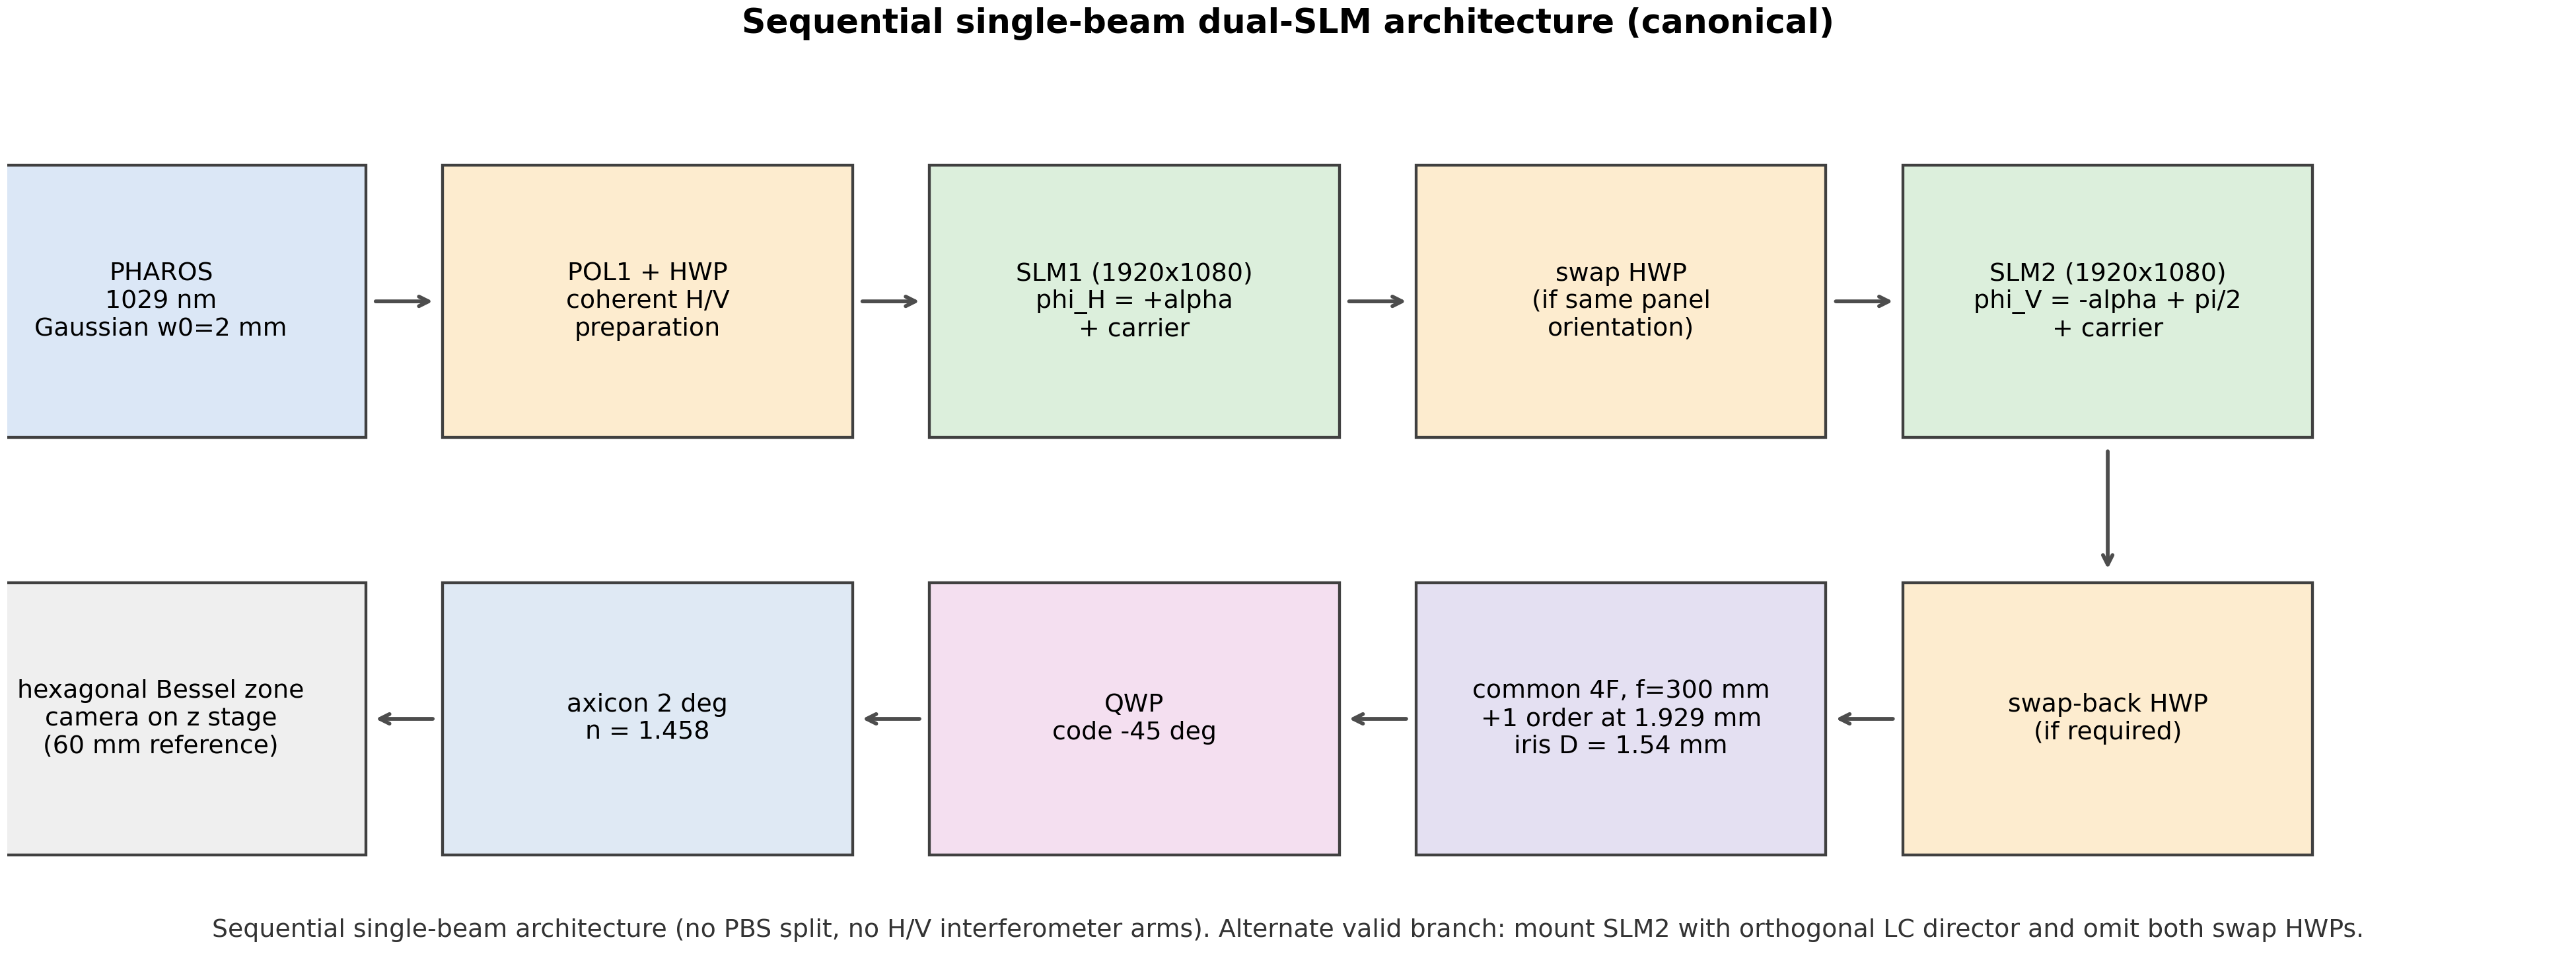
\includegraphics[width=\linewidth,height=0.86\textheight,keepaspectratio]{report/refined_figures/F1_sequential_architecture.png}
\caption{F1: Sequential single-beam dual-SLM architecture (canonical; no PBS split, no H/V interferometer arms).}
\end{figure}

\begin{figure}[p]
\centering
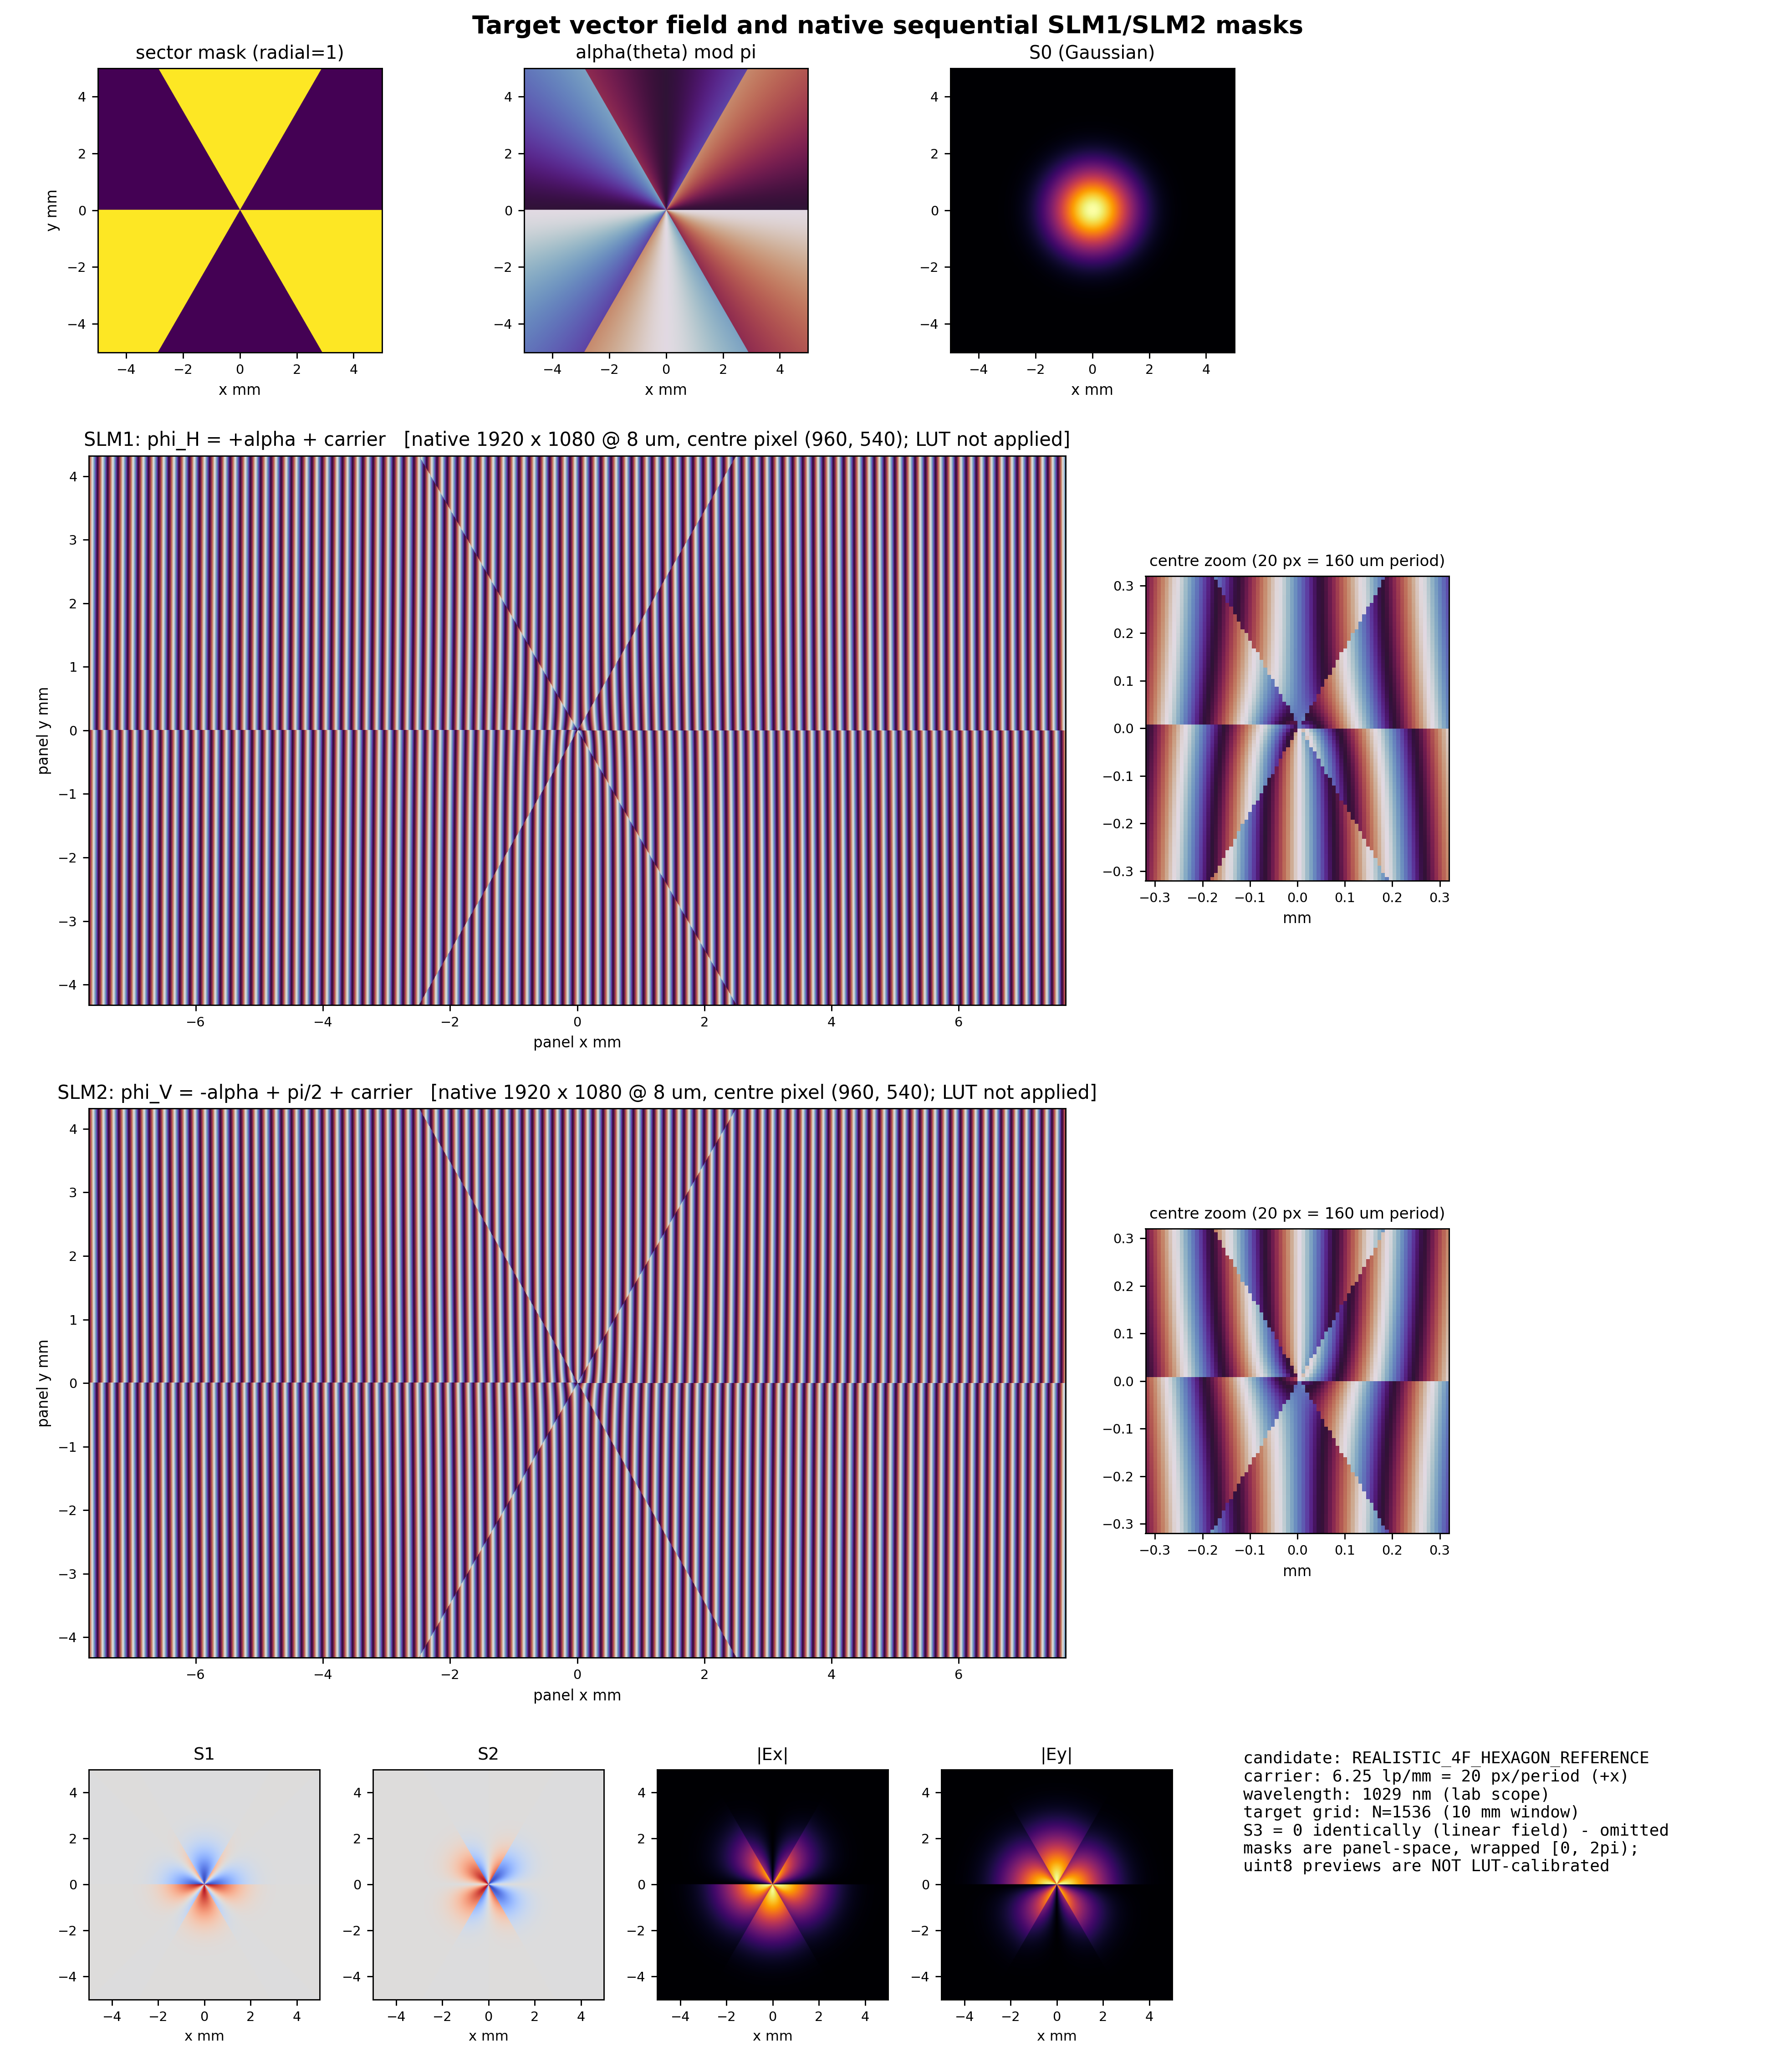
\includegraphics[width=\linewidth,height=0.86\textheight,keepaspectratio]{report/refined_figures/F2_target_and_masks.png}
\caption{F2: Target vector field and native sequential SLM1/SLM2 masks with centre carrier zoom (LUT not applied).}
\end{figure}

\begin{figure}[p]
\centering
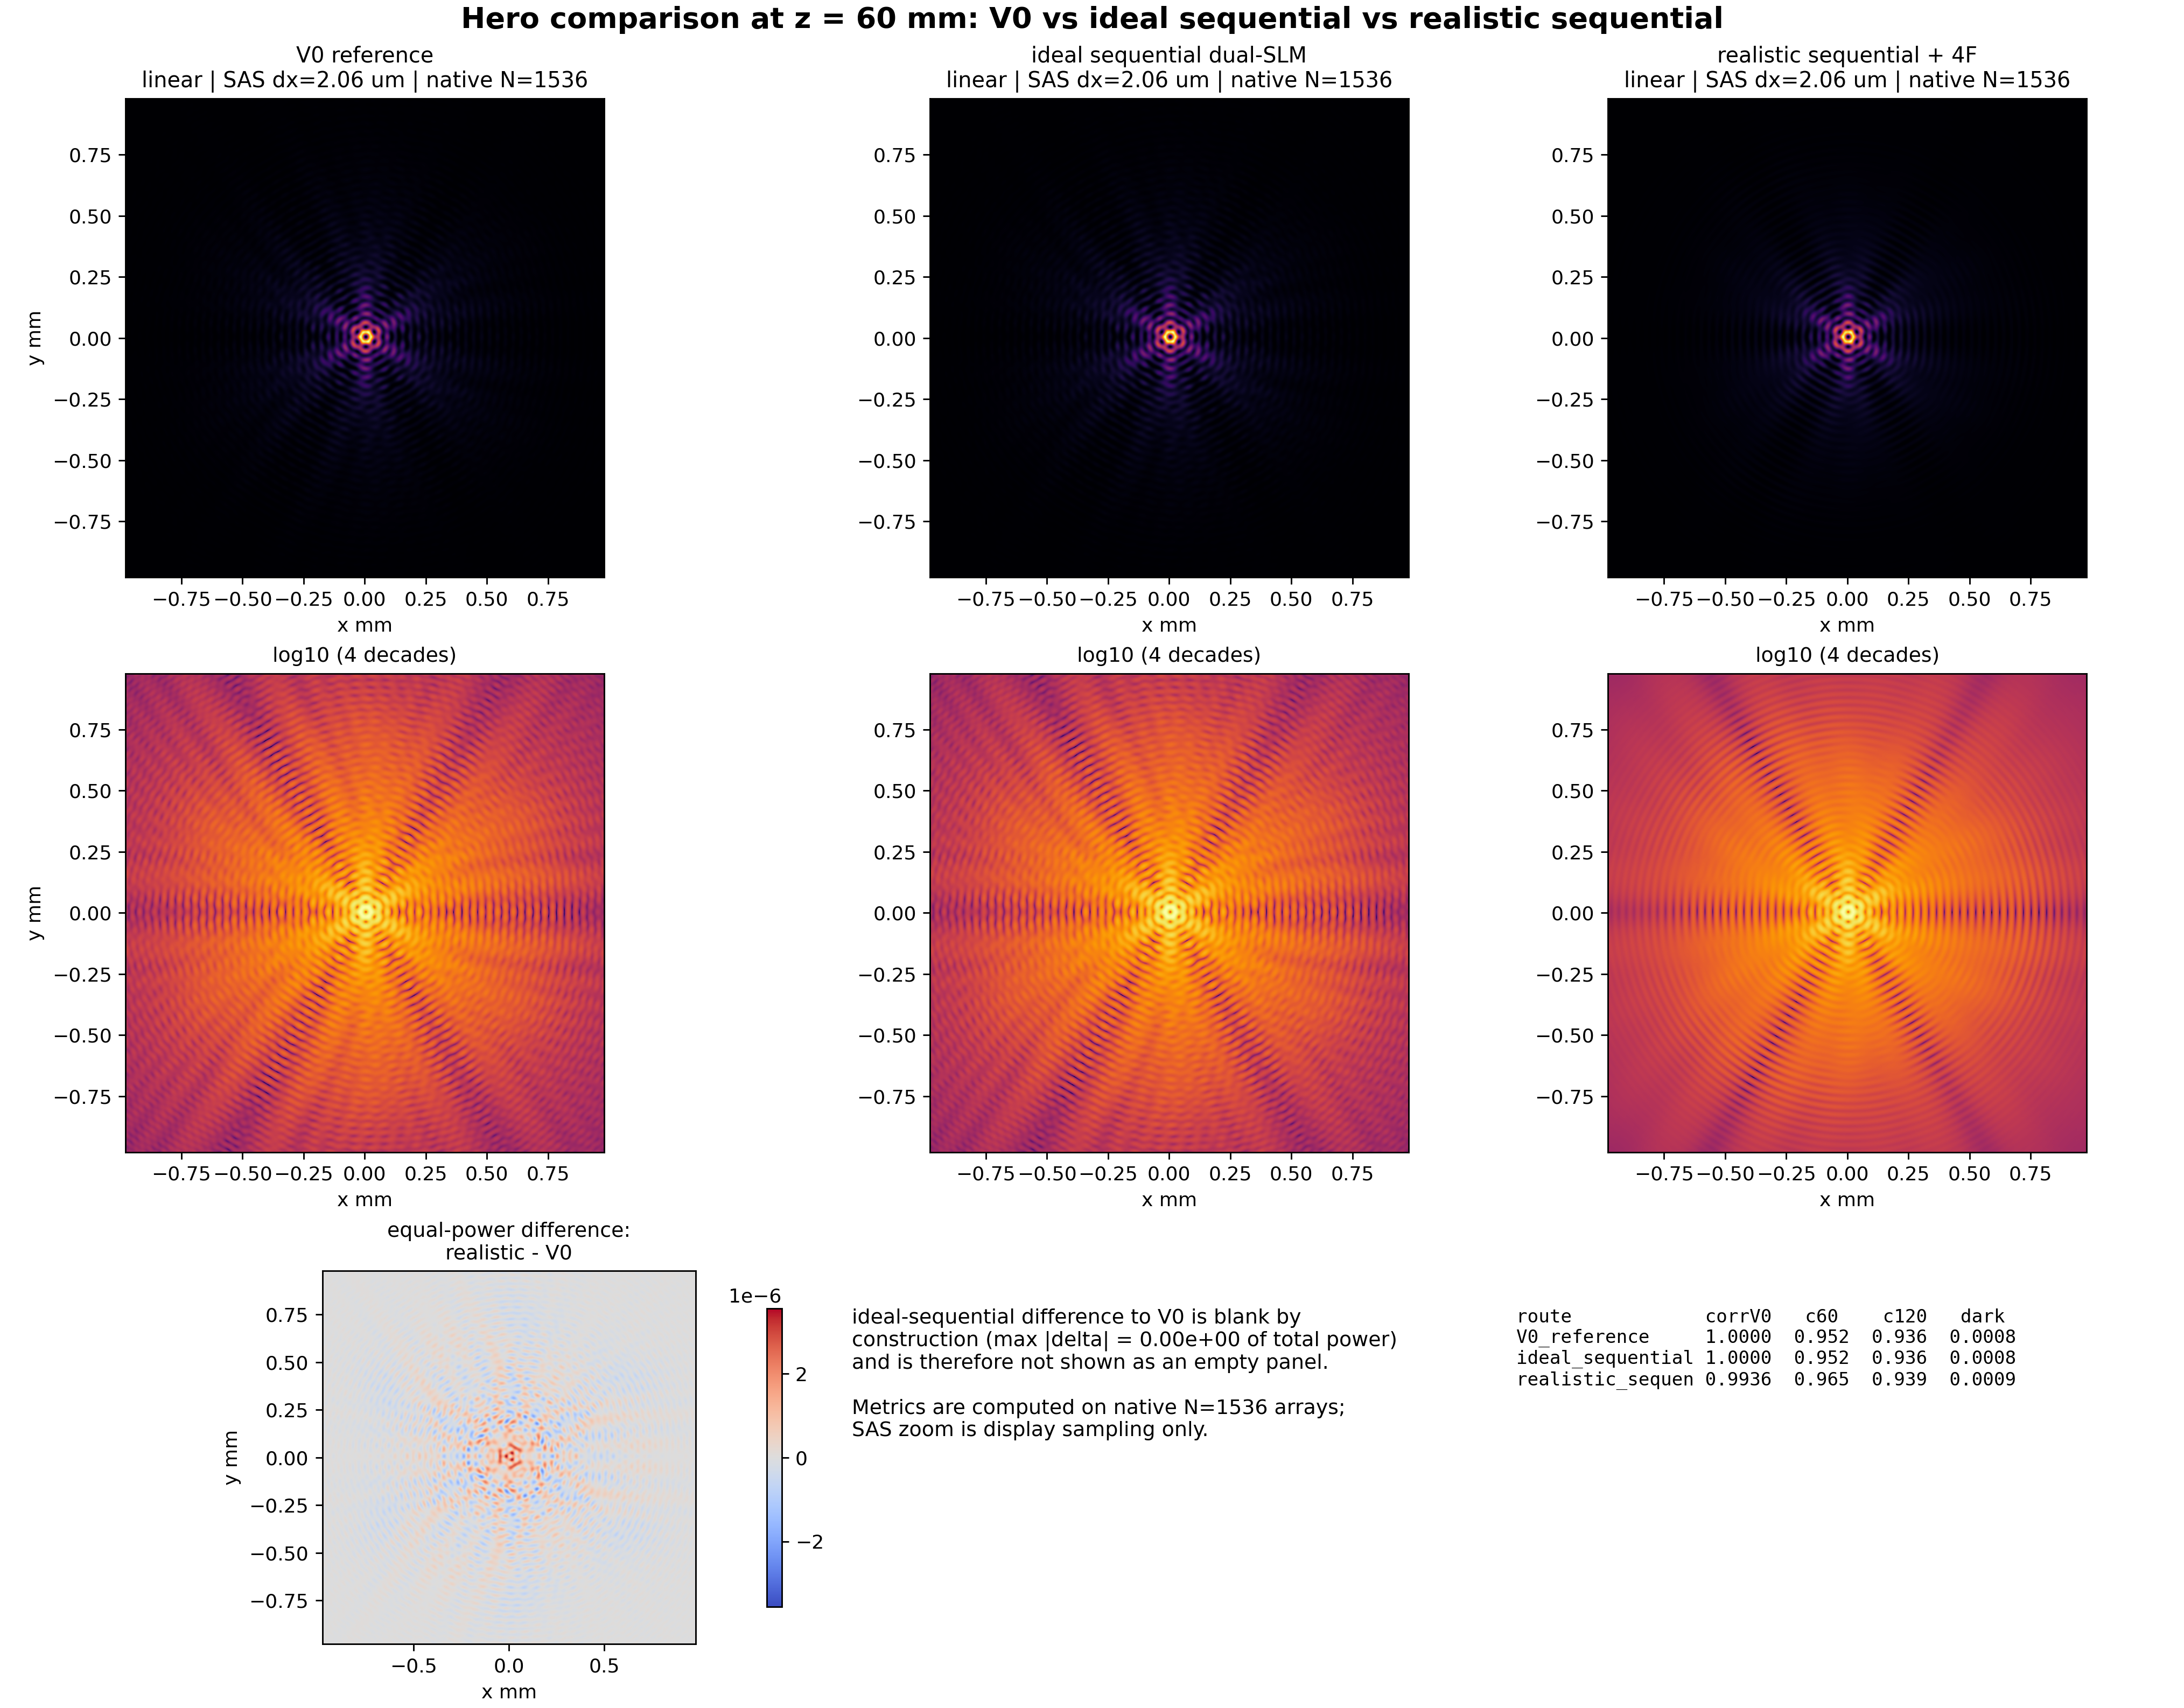
\includegraphics[width=\linewidth,height=0.86\textheight,keepaspectratio]{report/refined_figures/F3A_hero_comparison.png}
\caption{F3A: Hero comparison at z=60 mm: V0 versus ideal sequential versus realistic sequential (N=1536 native; SAS display sampling).}
\end{figure}

\begin{figure}[p]
\centering
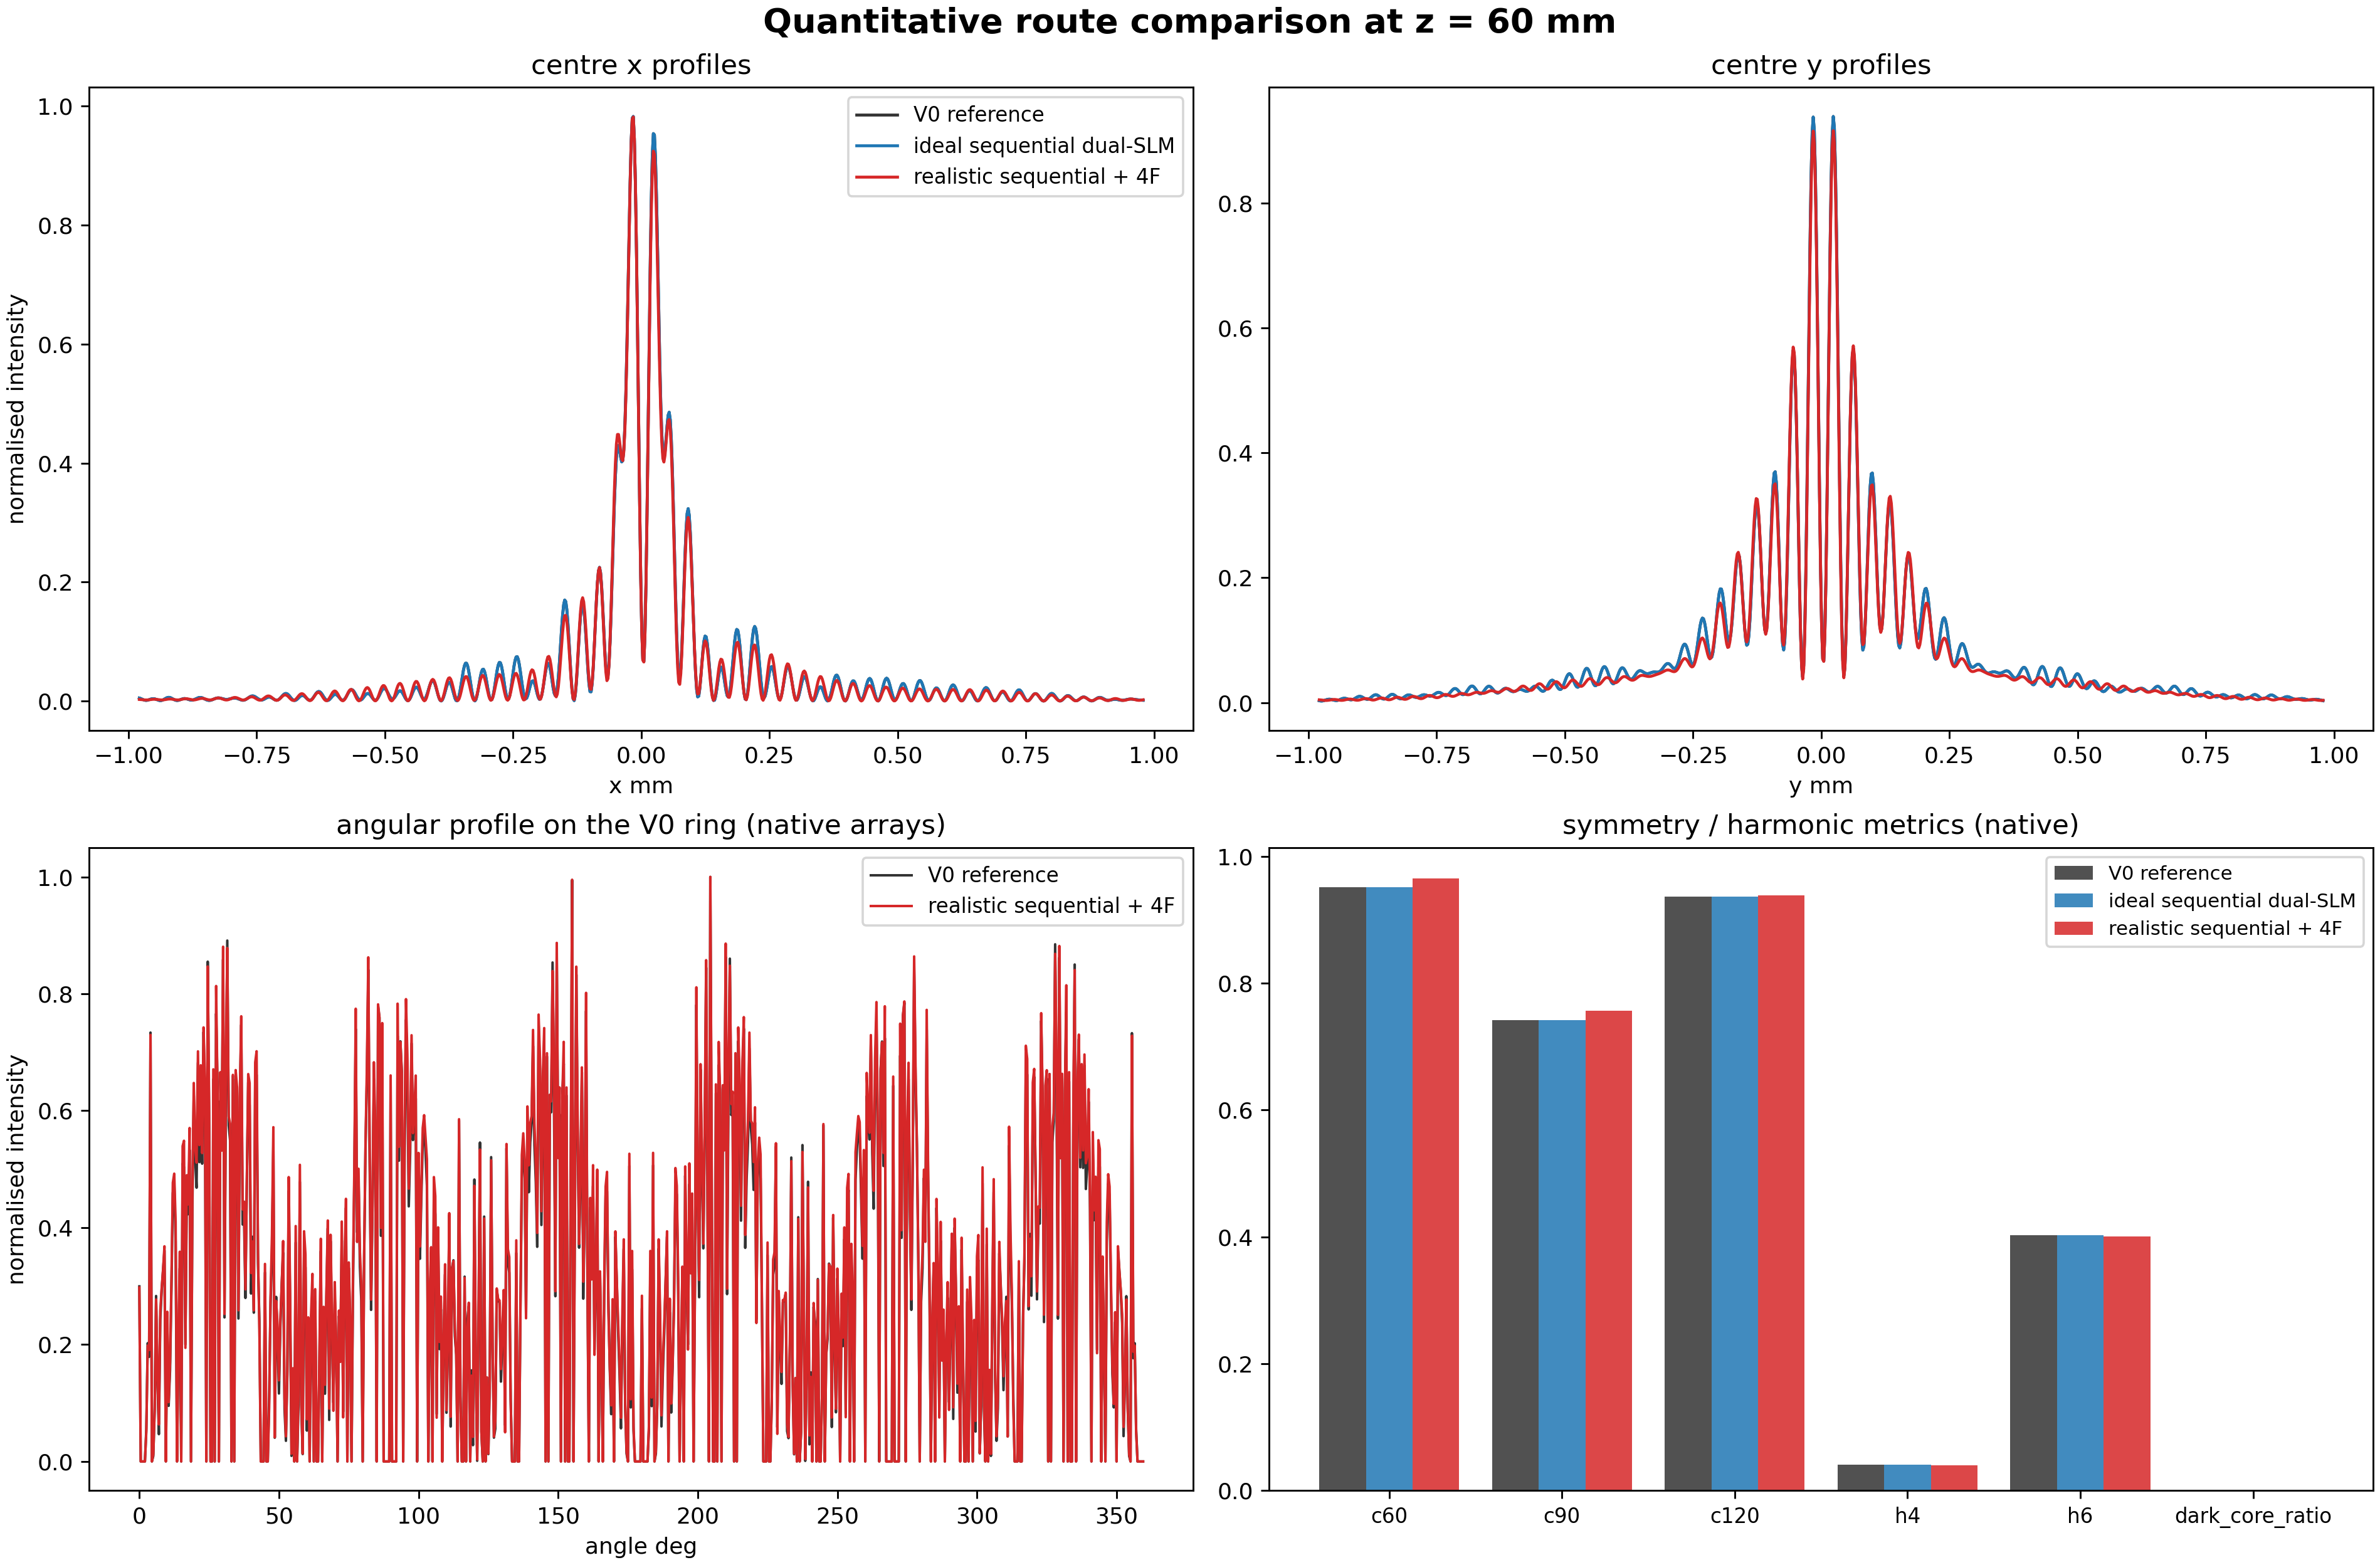
\includegraphics[width=\linewidth,height=0.86\textheight,keepaspectratio]{report/refined_figures/F3B_quantitative_comparison.png}
\caption{F3B: Quantitative route comparison: centre profiles, angular profile and symmetry/harmonic metrics.}
\end{figure}

\begin{figure}[p]
\centering
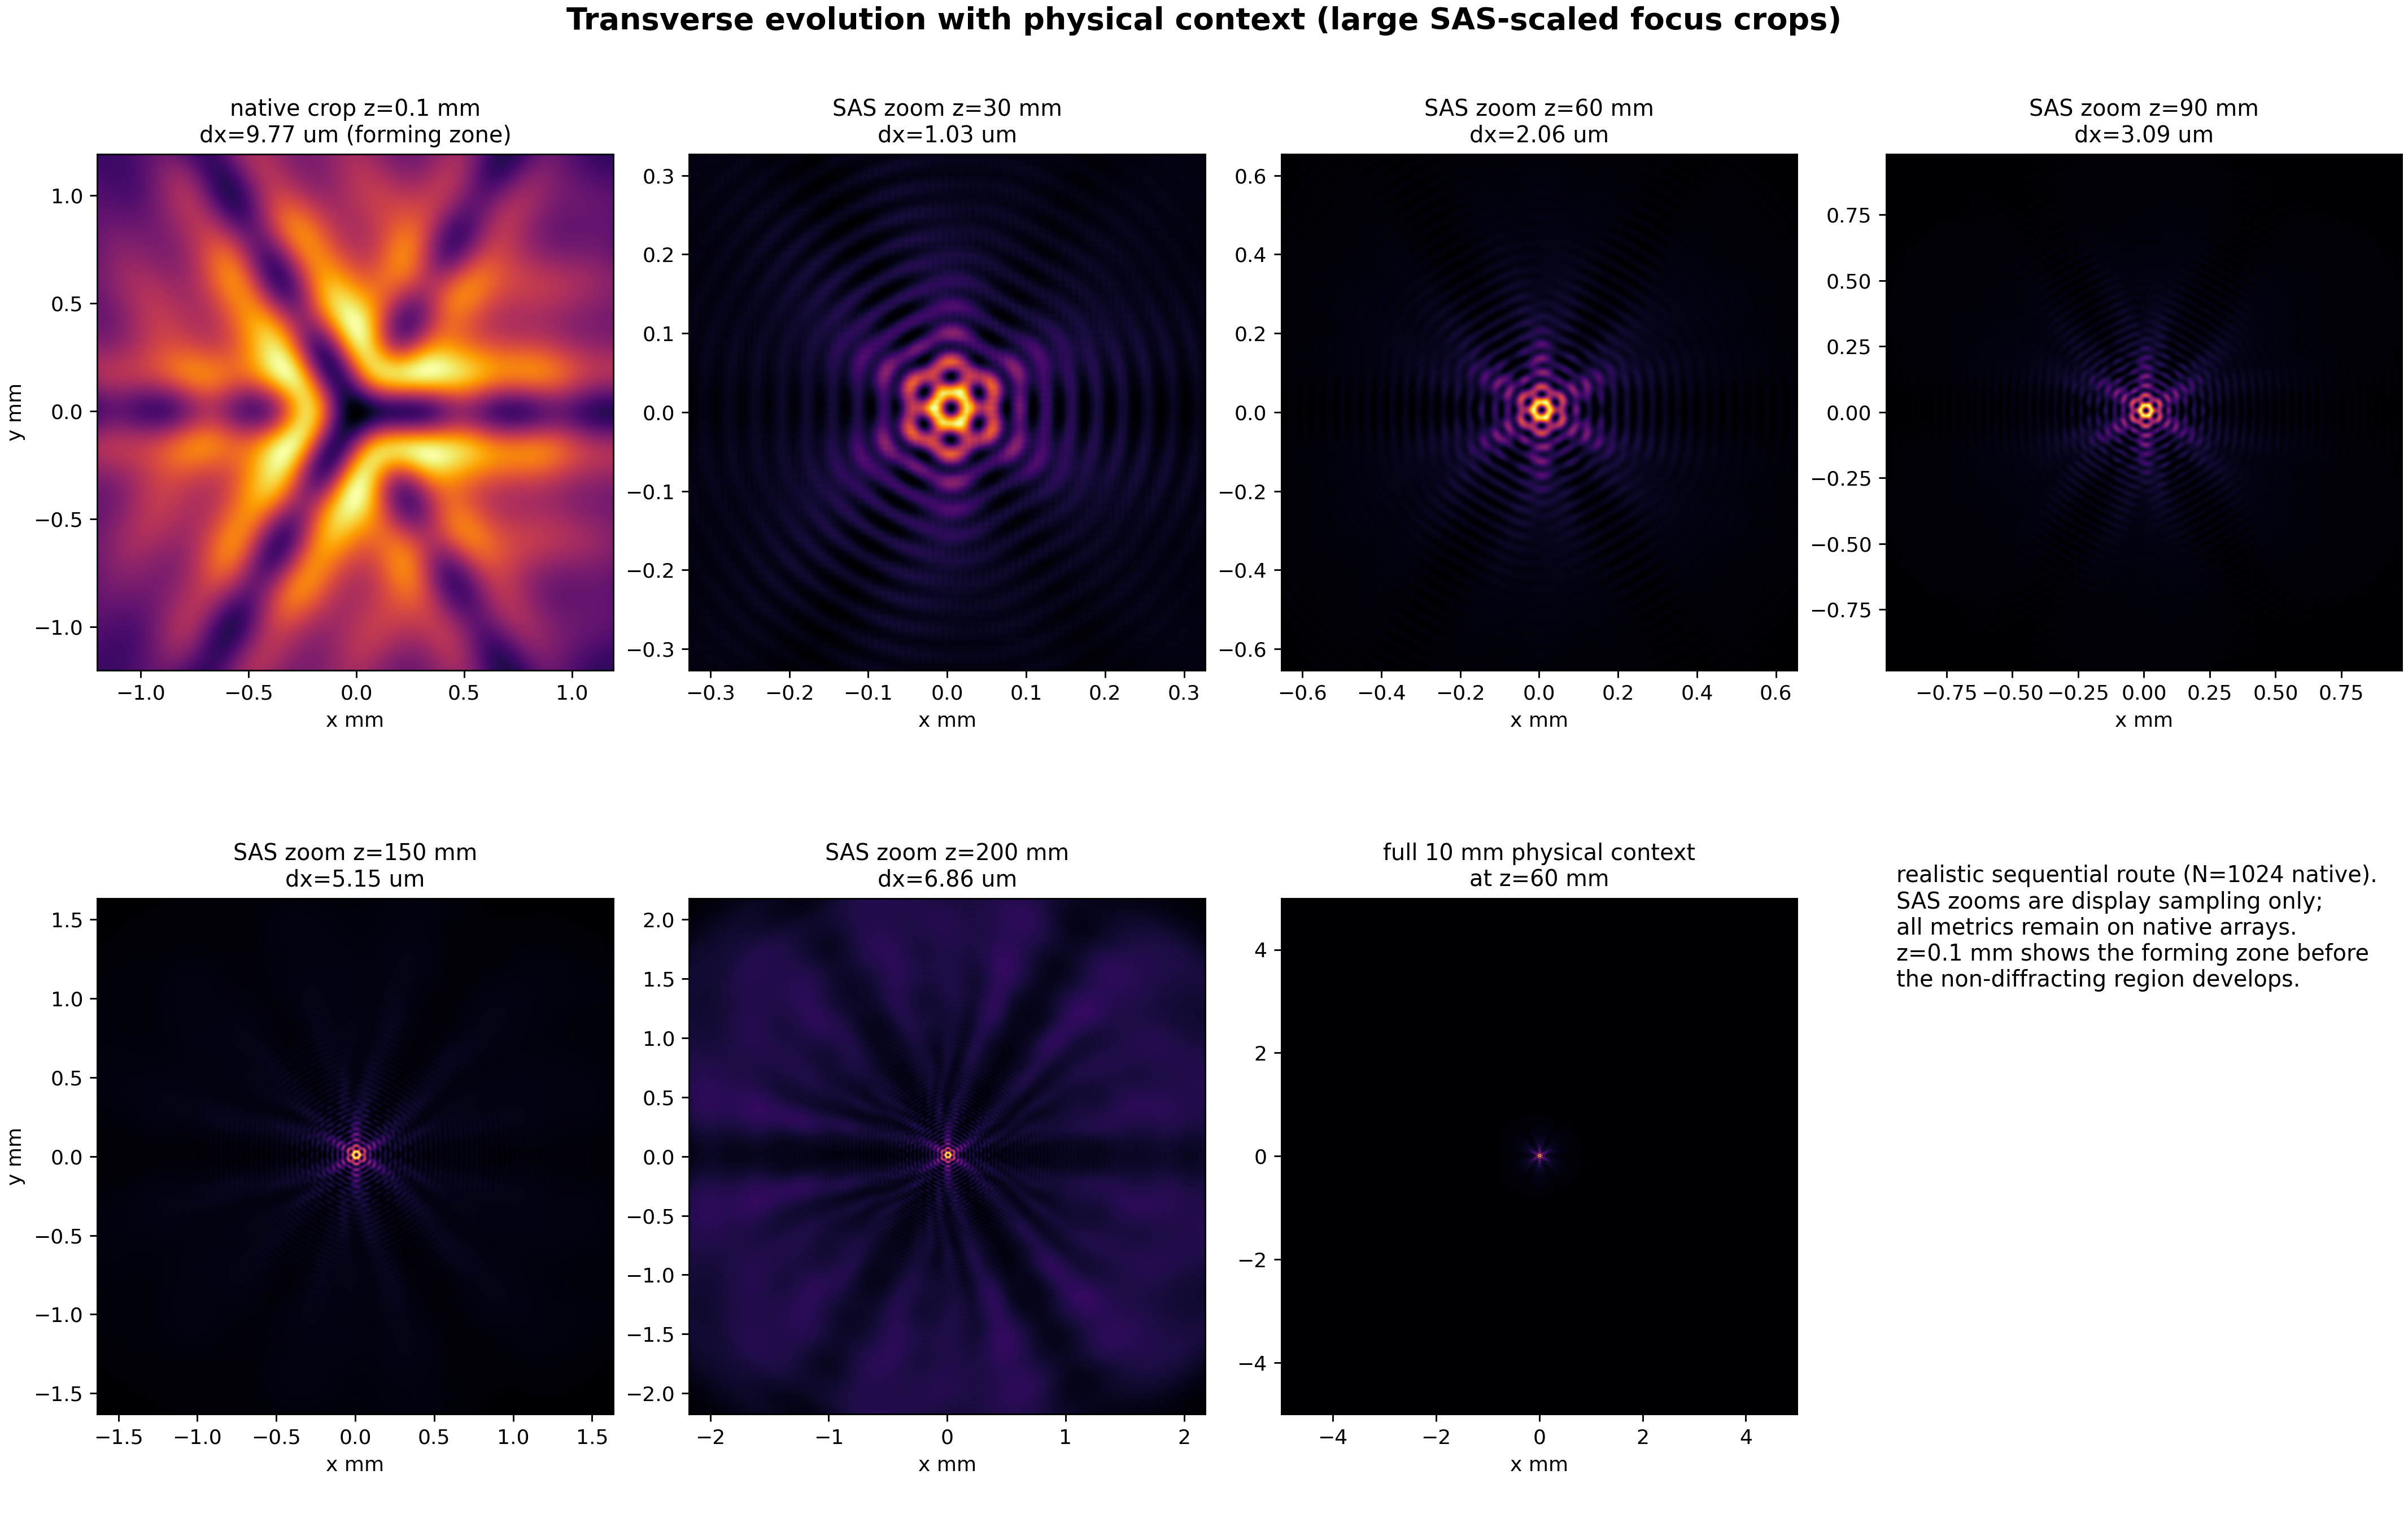
\includegraphics[width=\linewidth,height=0.86\textheight,keepaspectratio]{report/refined_figures/F4A_transverse_evolution.png}
\caption{F4A: Transverse evolution with physical context and large SAS-scaled focus crops (realistic sequential route).}
\end{figure}

\begin{figure}[p]
\centering
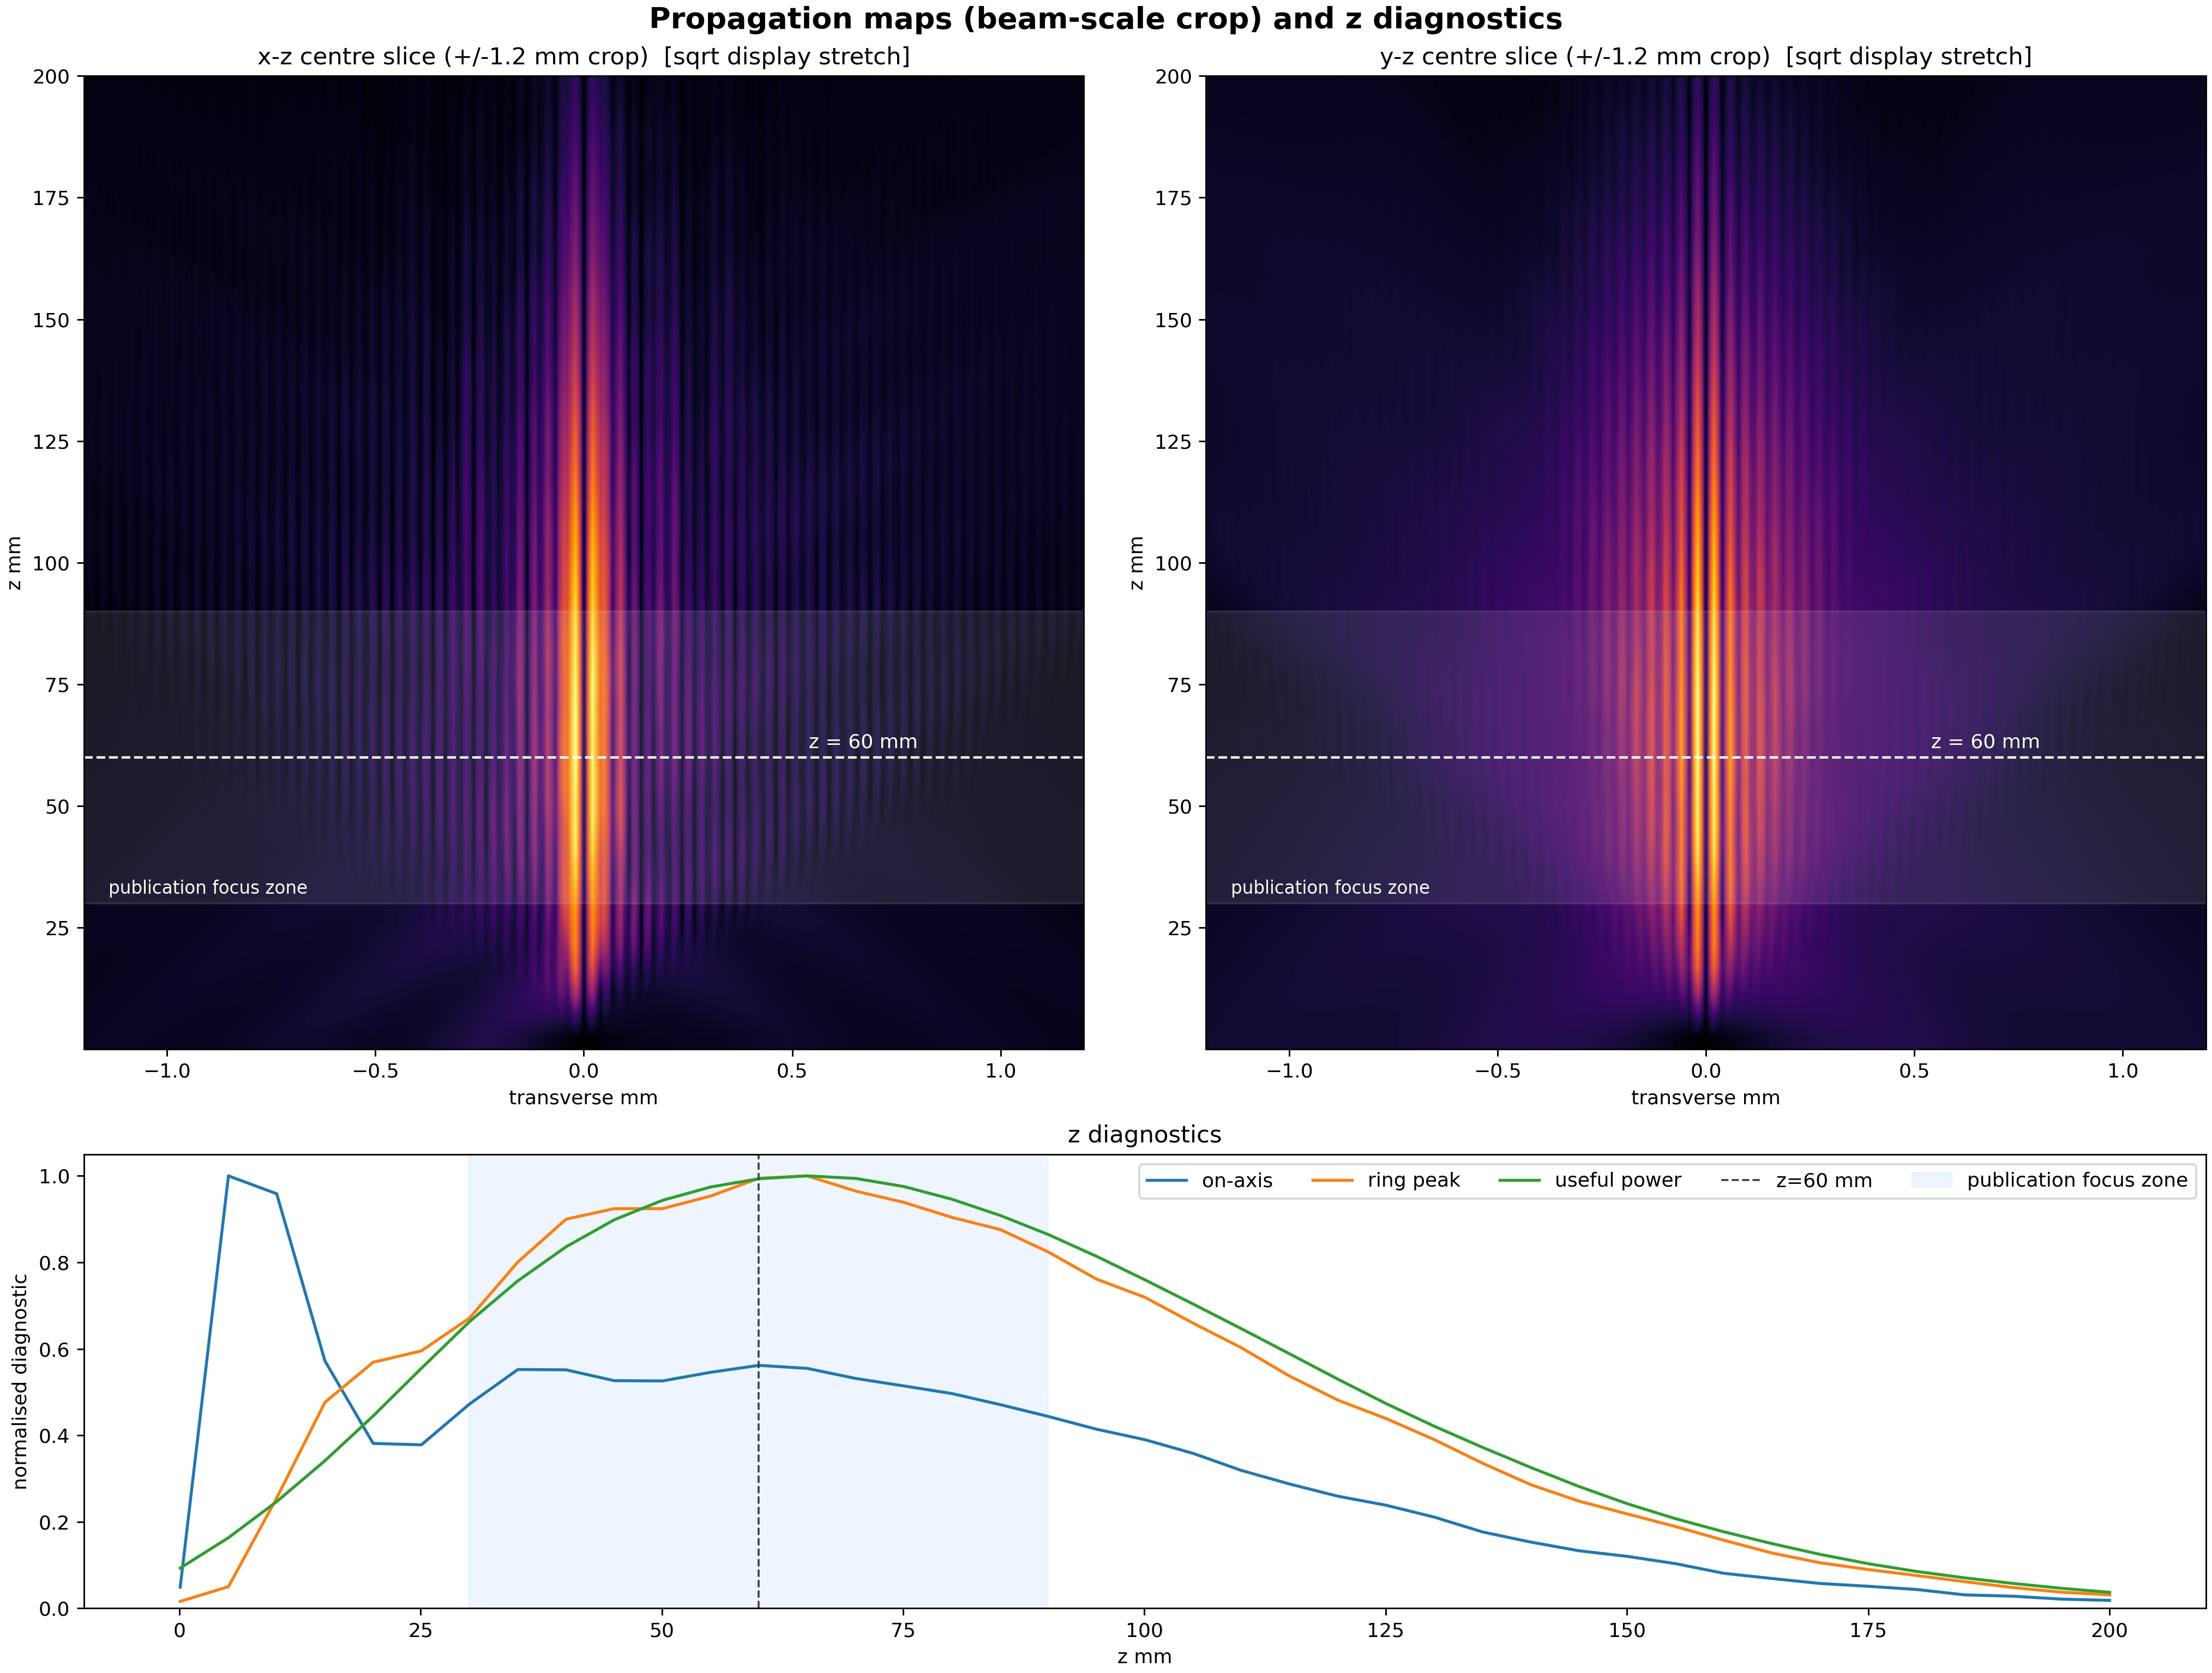
\includegraphics[width=\linewidth,height=0.86\textheight,keepaspectratio]{report/refined_figures/F4B_xz_yz_propagation.png}
\caption{F4B: Propagation maps cropped to the beam scale (+/-1.2 mm) with z diagnostics; z=60 mm and the focus zone marked.}
\end{figure}

\begin{figure}[p]
\centering
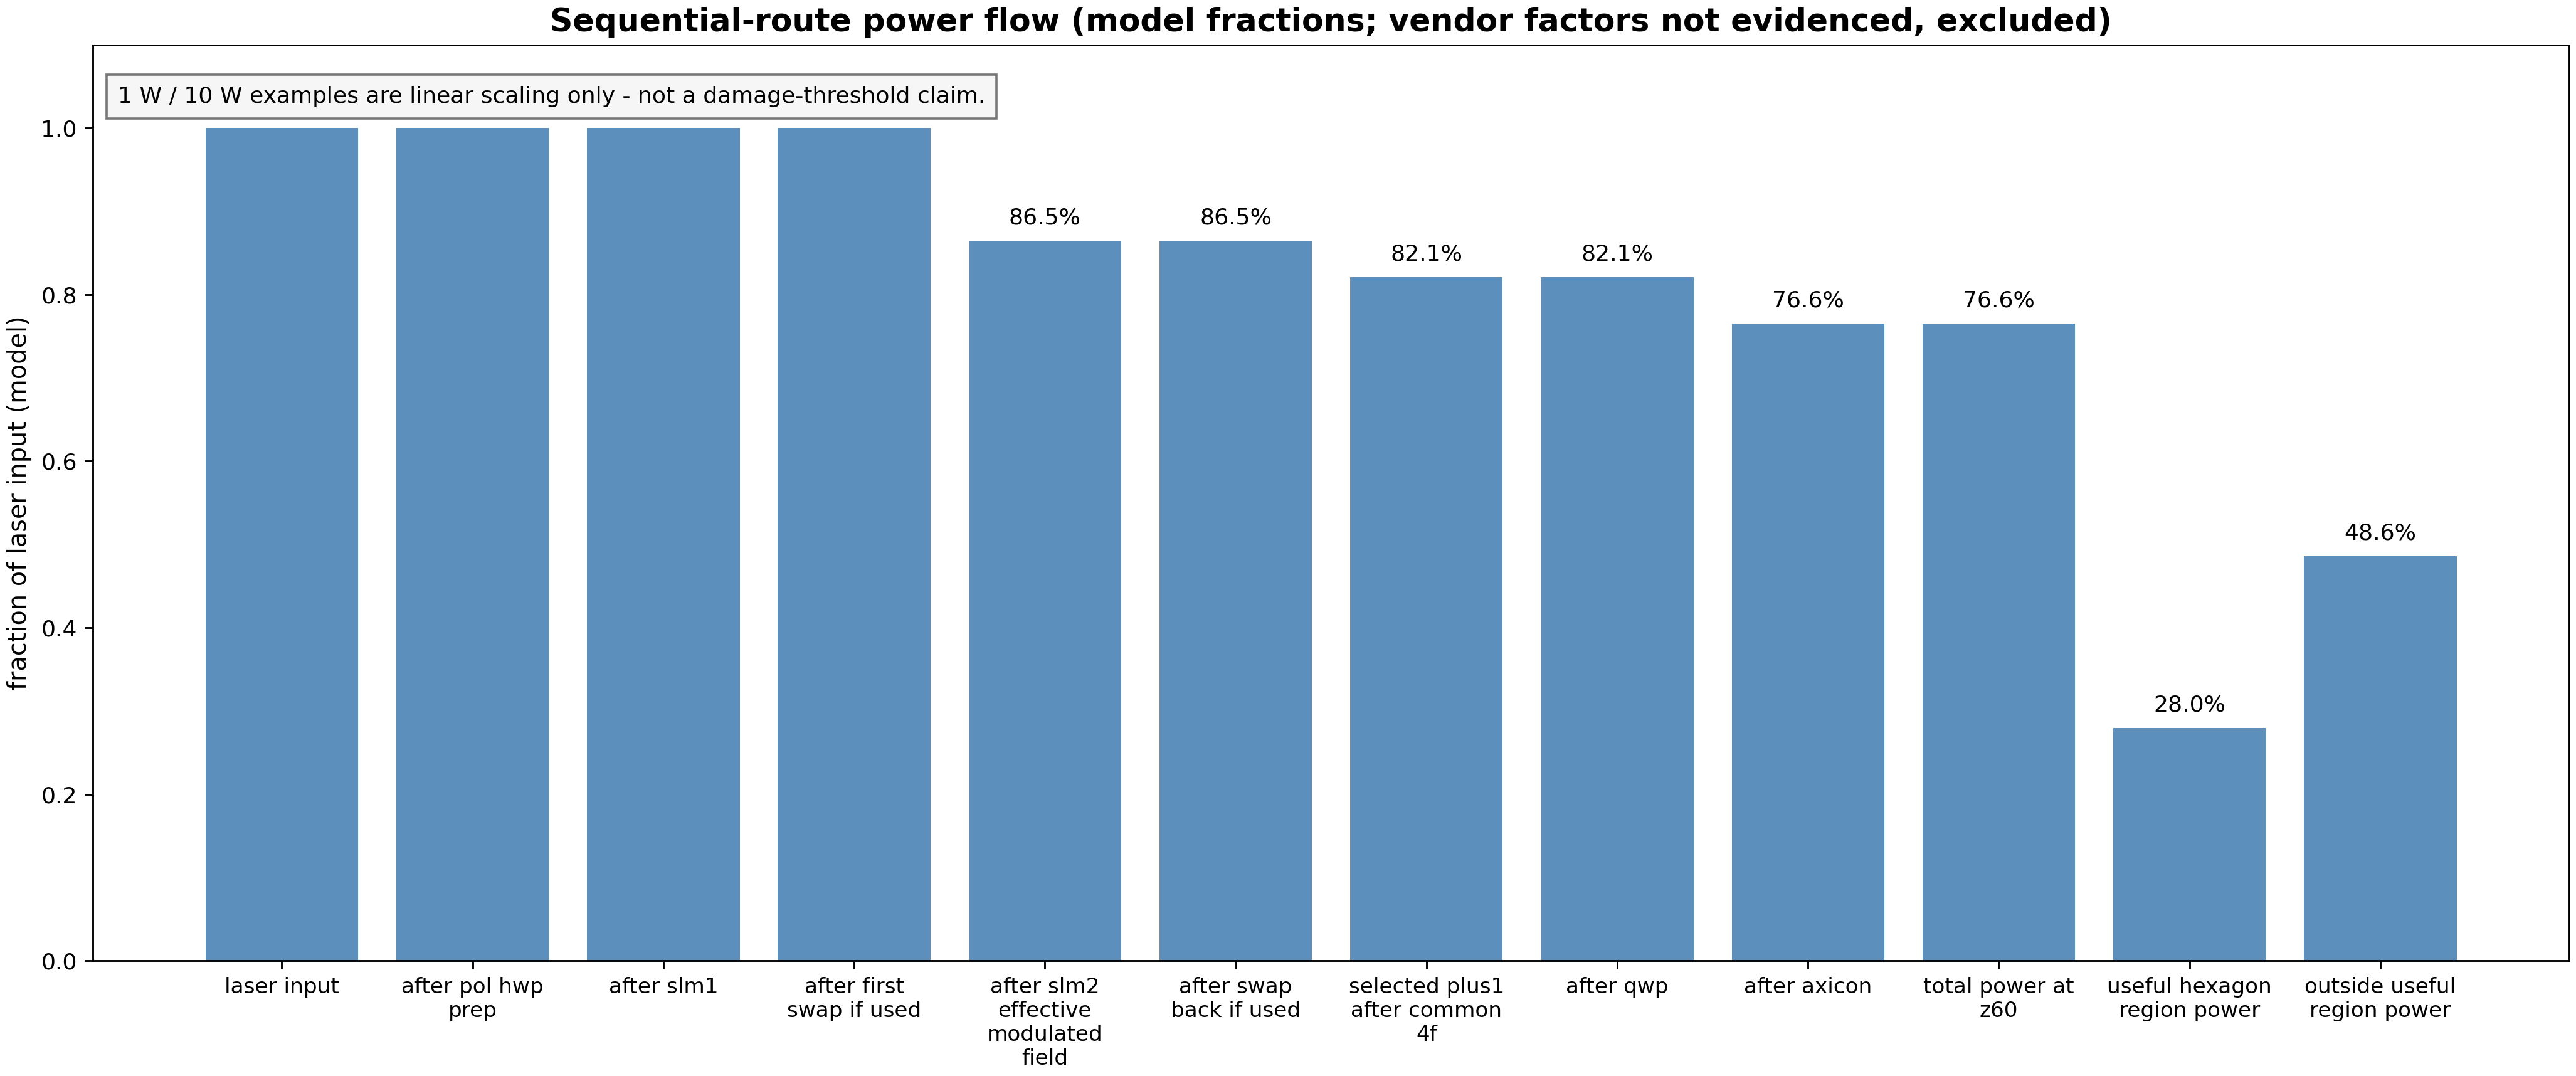
\includegraphics[width=\linewidth,height=0.86\textheight,keepaspectratio]{report/refined_figures/F4C_sequential_power_flow.png}
\caption{F4C: Sequential-route power flow (model fractions; linear power-scaling examples are not damage-threshold claims).}
\end{figure}

\begin{figure}[p]
\centering
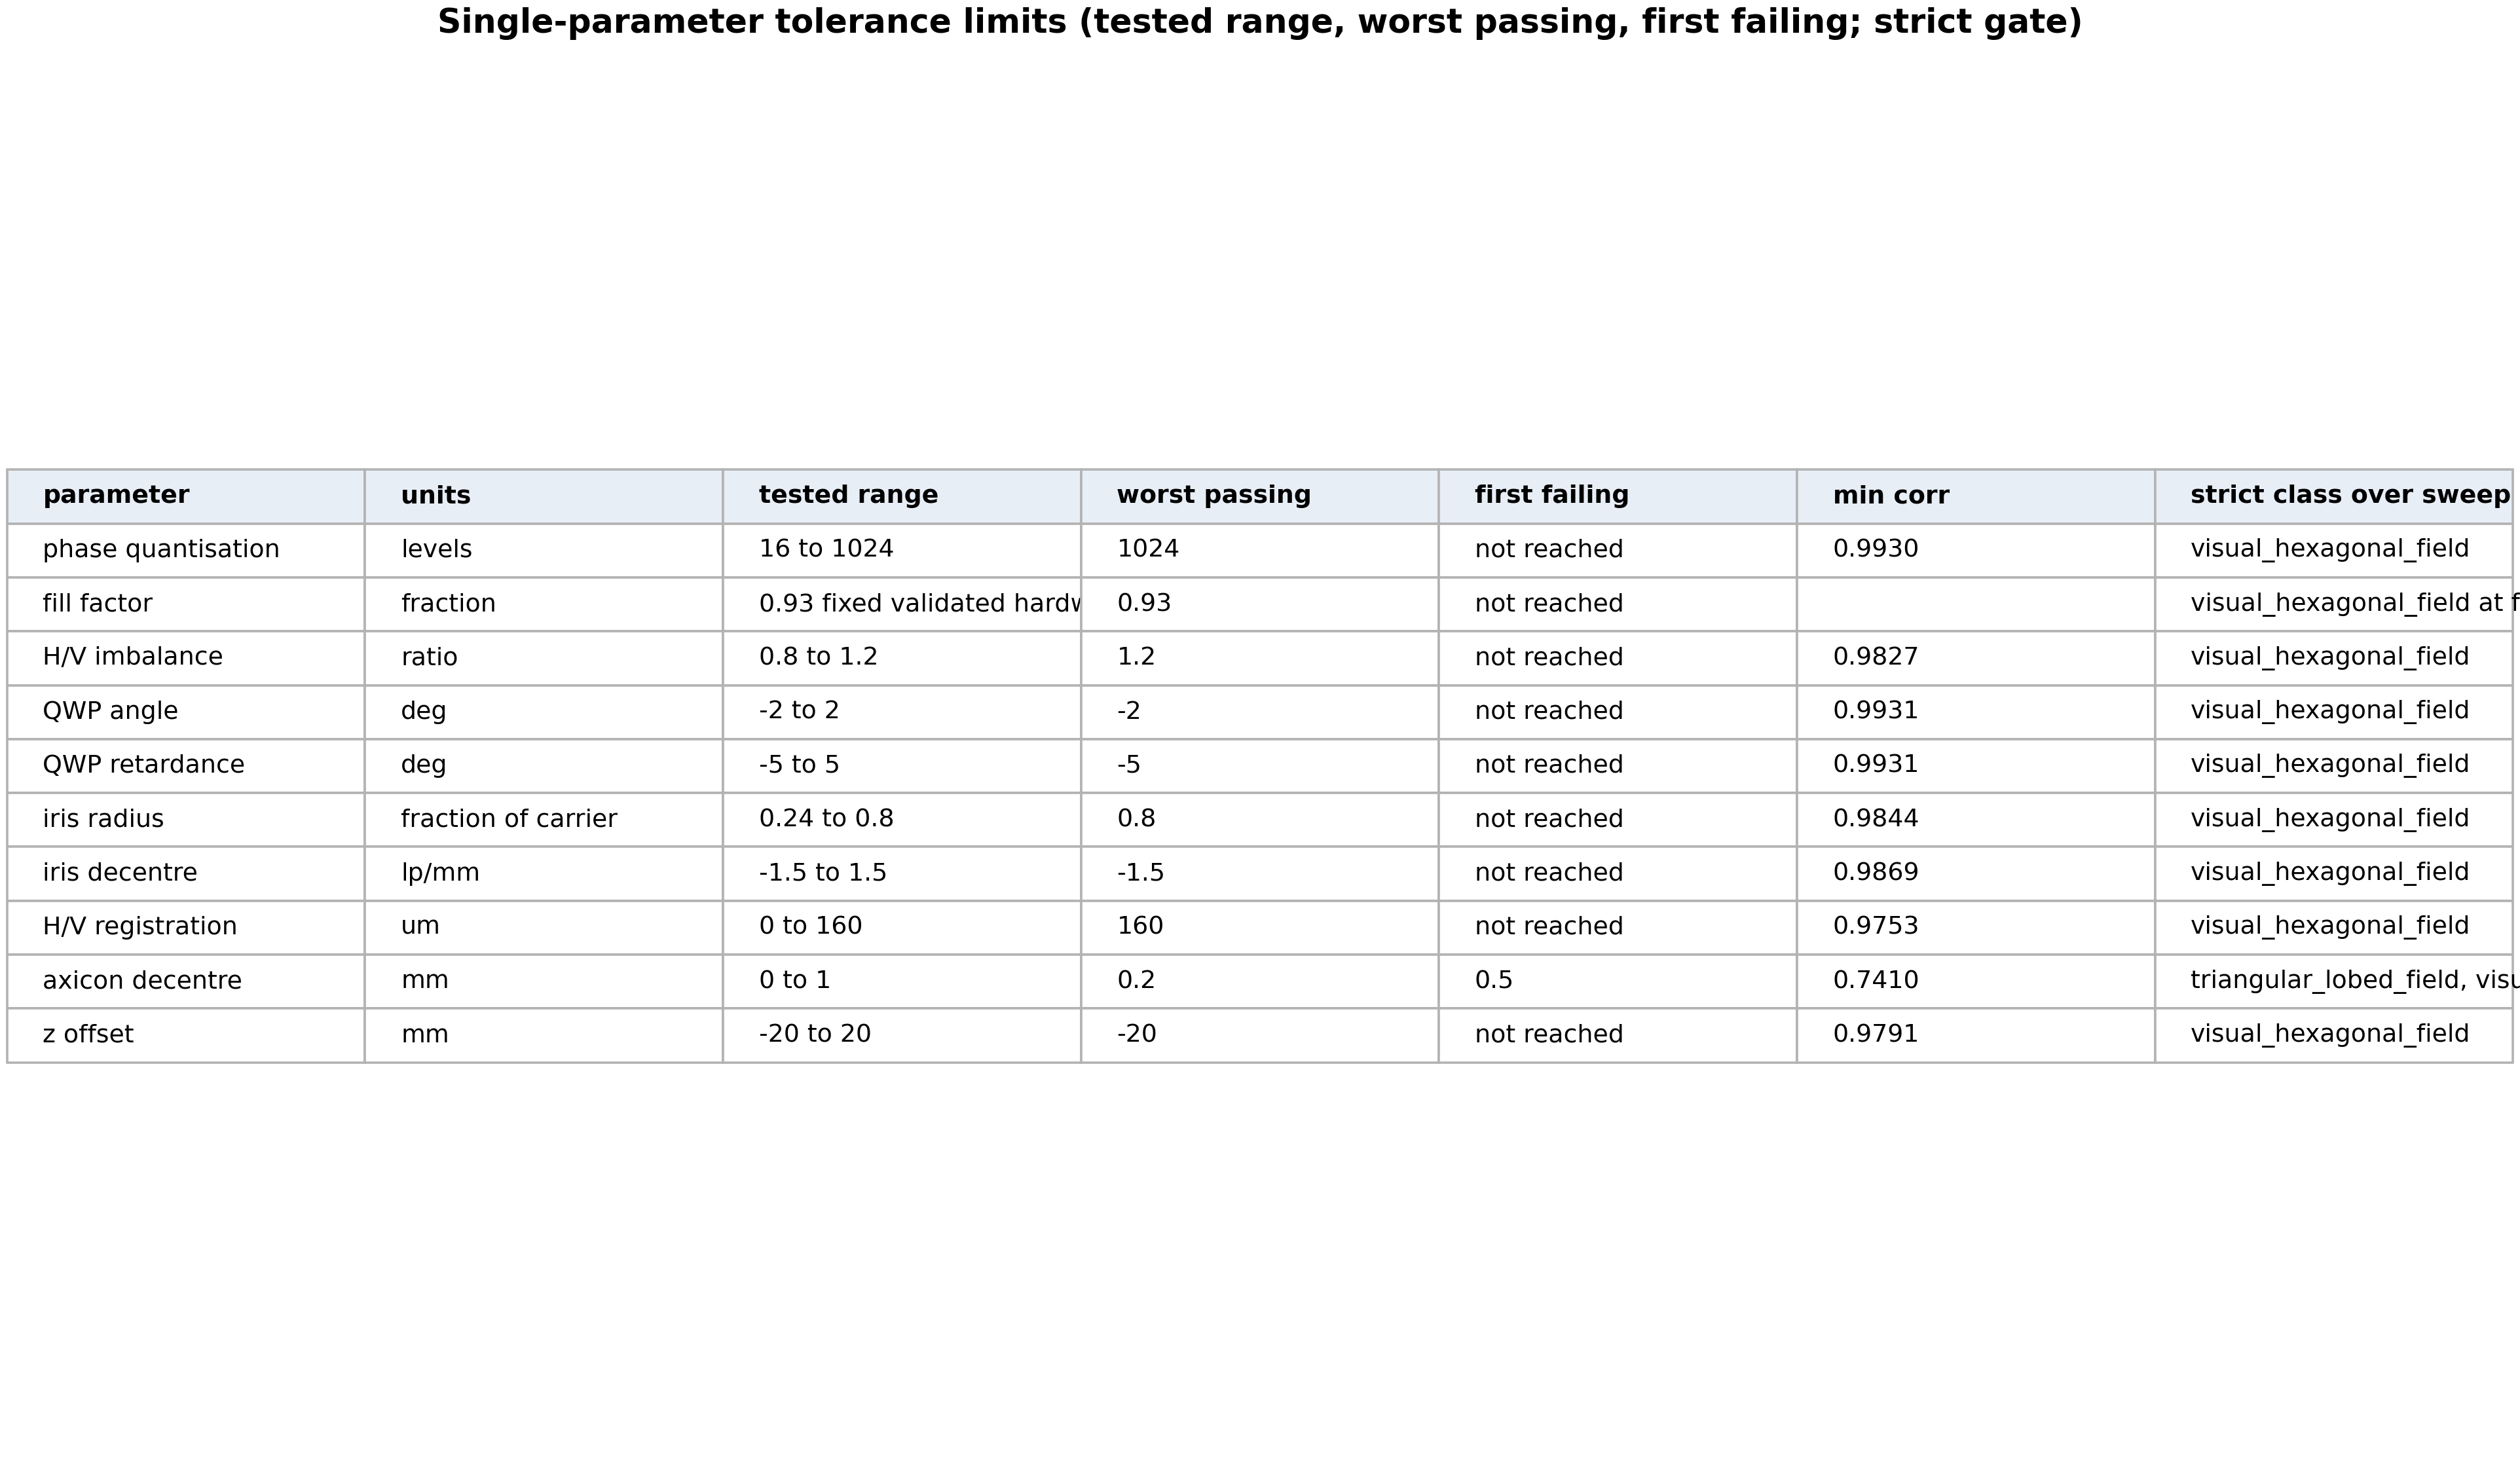
\includegraphics[width=\linewidth,height=0.86\textheight,keepaspectratio]{report/refined_figures/F5A_tolerance_limits.png}
\caption{F5A: Single-parameter tolerance limits: tested range, worst passing value, first failing value and strict class.}
\end{figure}

\begin{figure}[p]
\centering
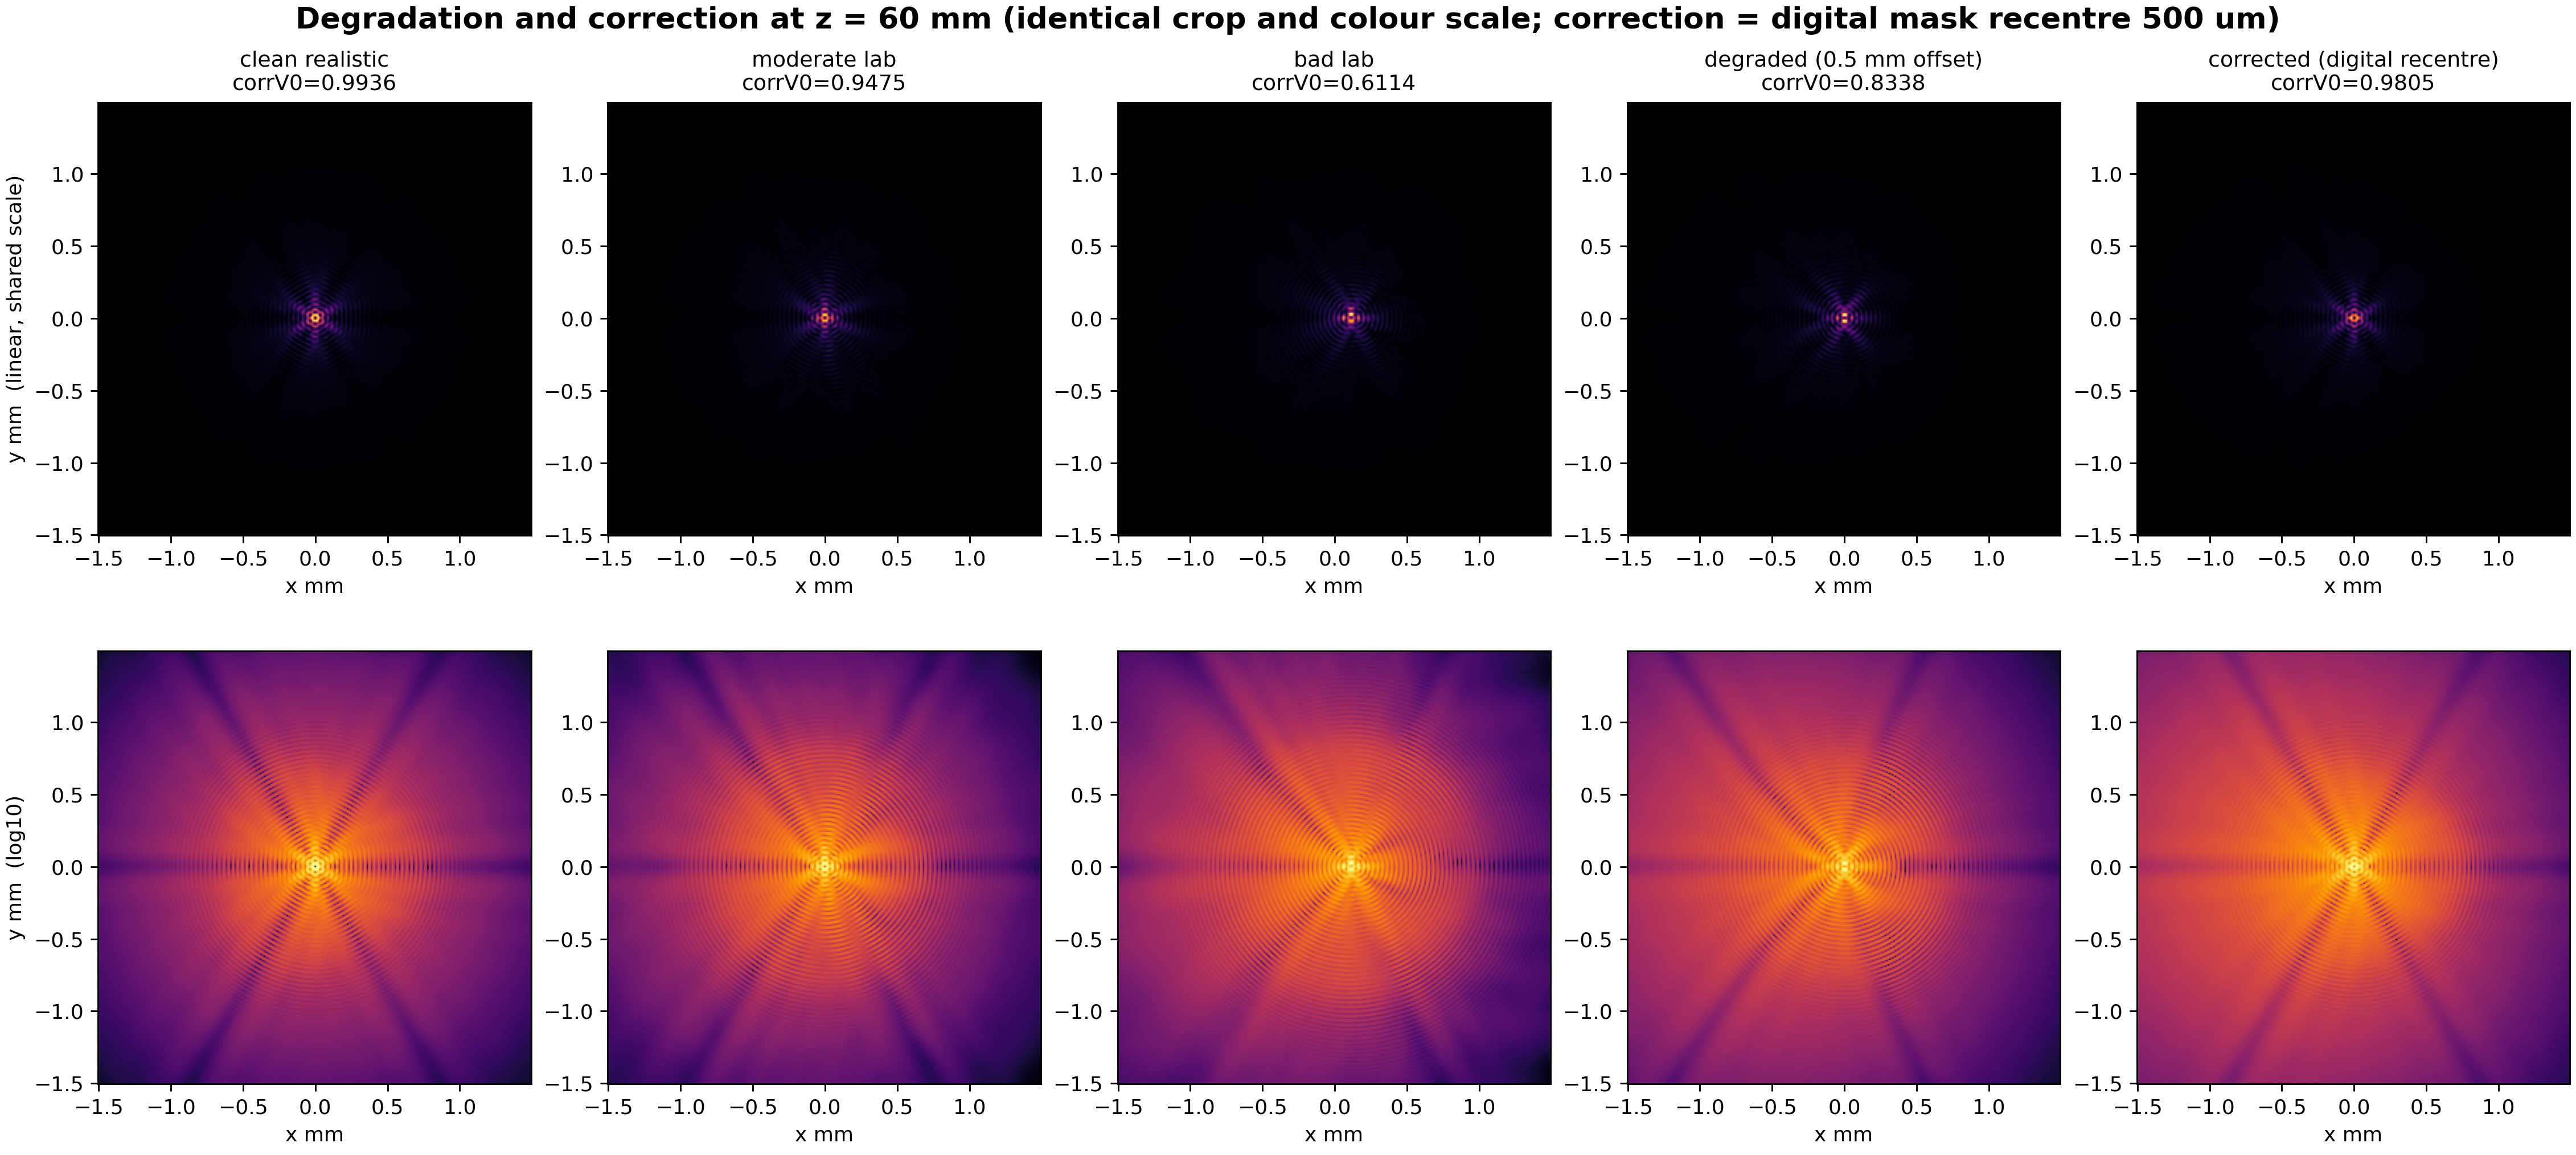
\includegraphics[width=\linewidth,height=0.86\textheight,keepaspectratio]{report/refined_figures/F5B_degradation_correction.png}
\caption{F5B: Degradation and correction at identical crop and colour scale: clean, moderate, bad, degraded and digitally recentred.}
\end{figure}

\begin{figure}[p]
\centering
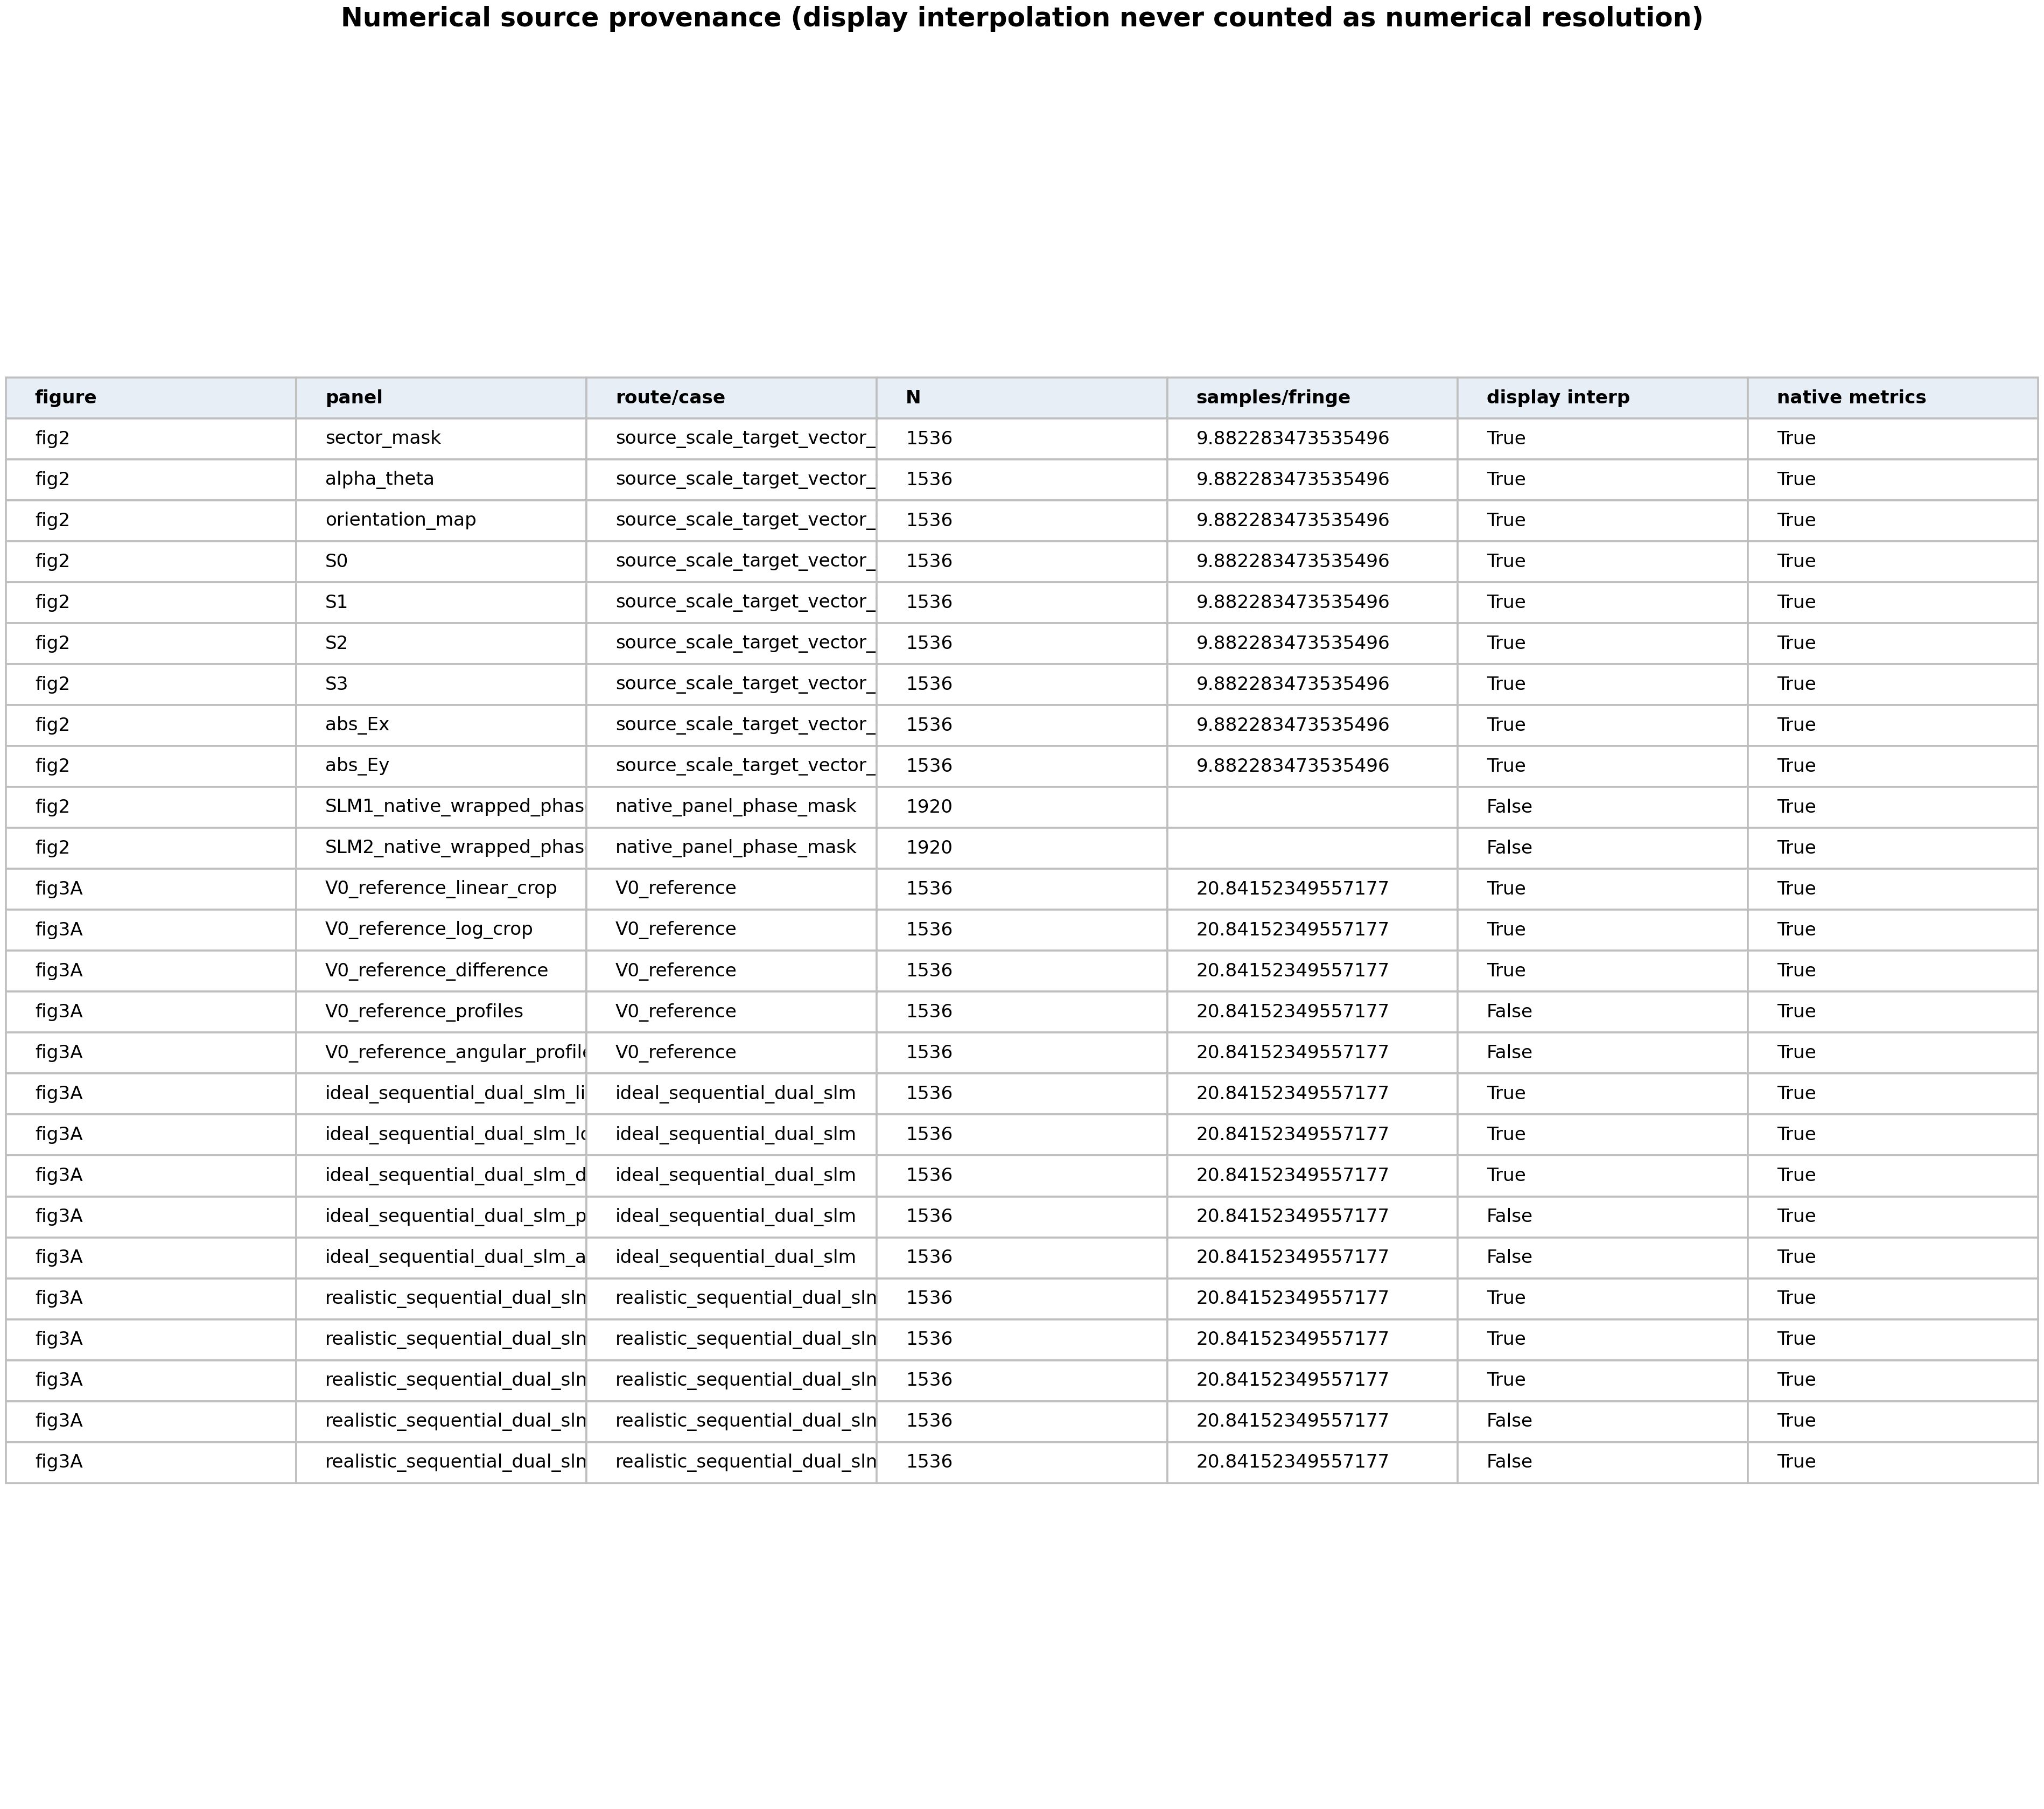
\includegraphics[width=\linewidth,height=0.86\textheight,keepaspectratio]{report/refined_figures/FA1_provenance_table.png}
\caption{FA1: Numerical source provenance: display interpolation is never counted as numerical resolution.}
\end{figure}

\appendix
\section{Audit and Superseded Evidence}
Dense audit composites and superseded material retained for provenance; see report/report\_visual\_audit.csv.
\begin{figure}[p]
\centering
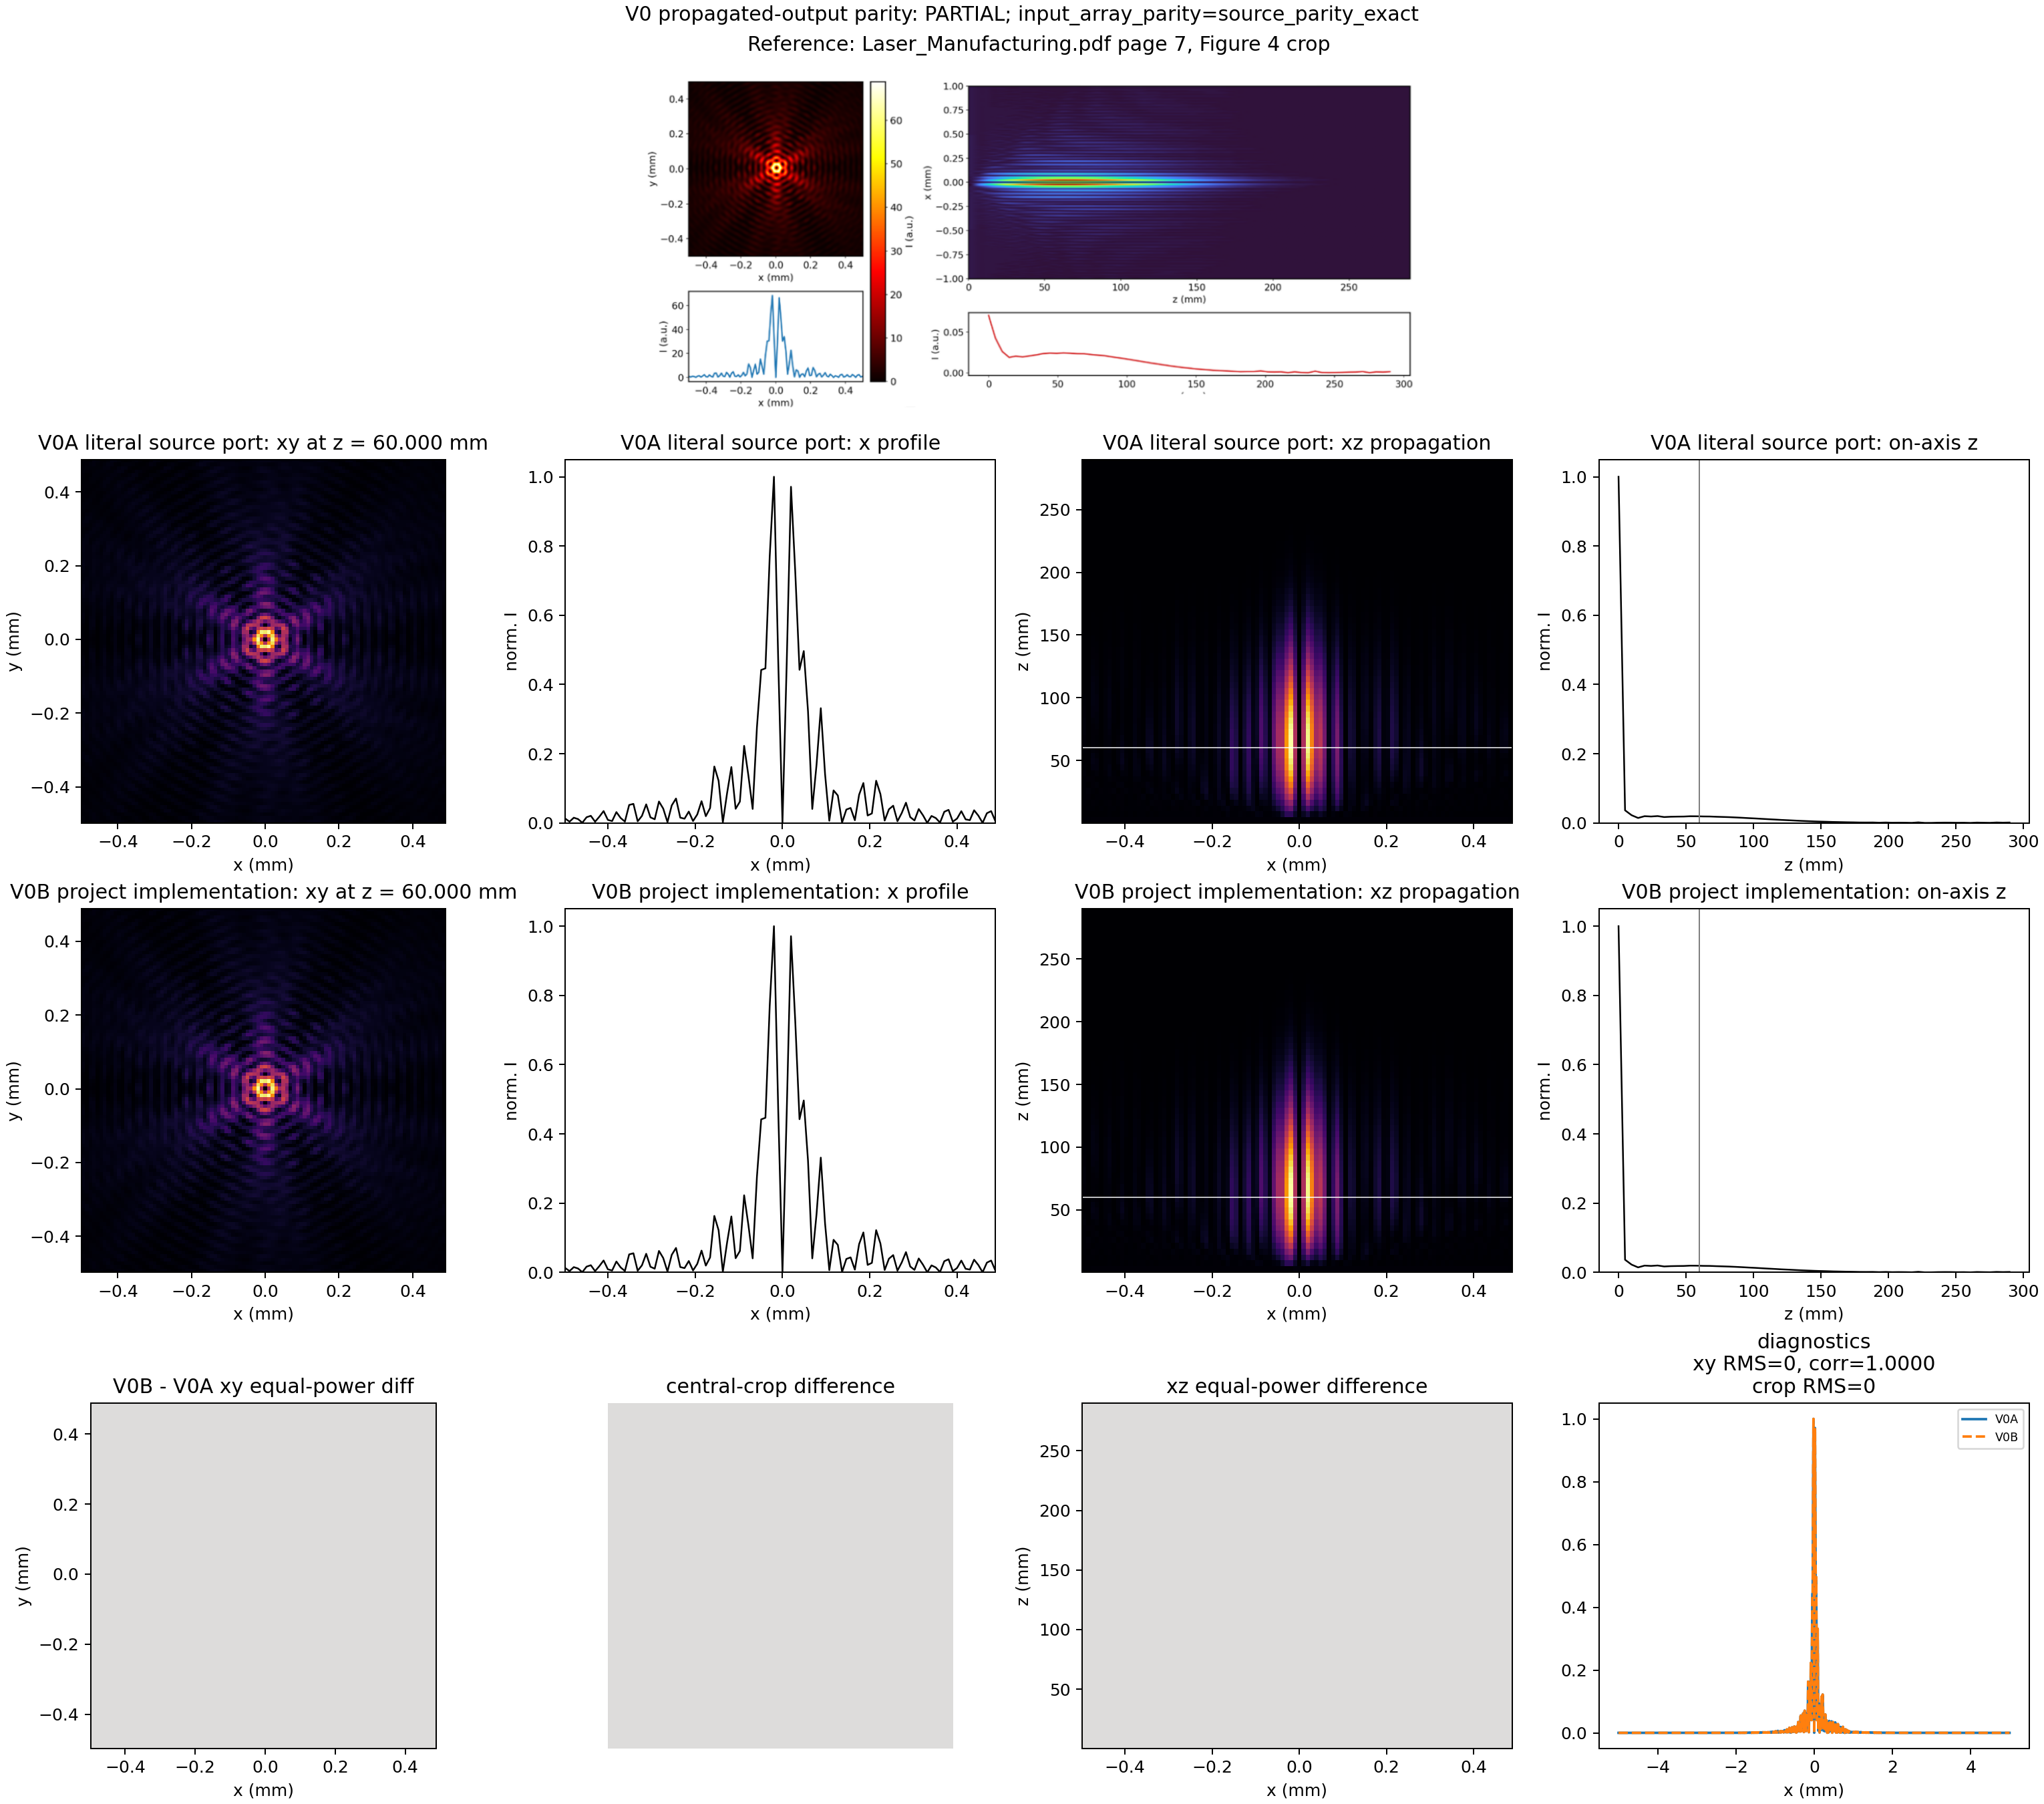
\includegraphics[width=\linewidth,height=0.82\textheight,keepaspectratio]{report/evidence_pack/source_validation/F01_nathan_visual_ladder_v0_reference_vs_reproduction.png}
\caption{F01 (appendix): V0 source parity and reference/reproduction comparison.}
\end{figure}

\begin{figure}[p]
\centering
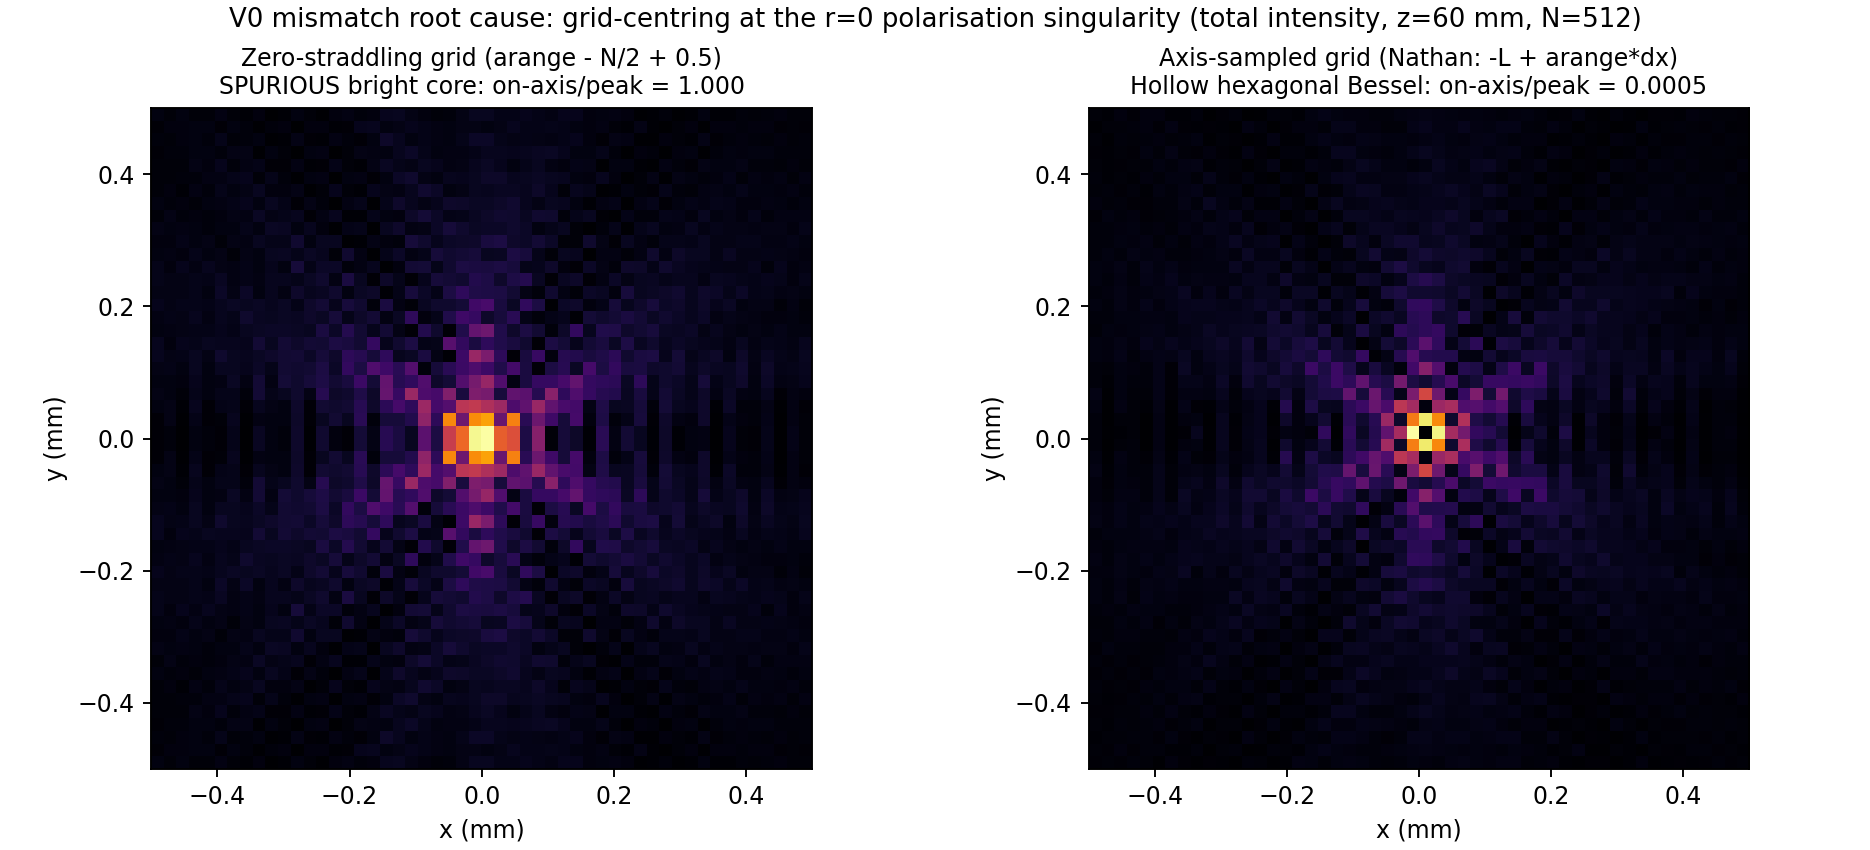
\includegraphics[width=\linewidth,height=0.82\textheight,keepaspectratio]{report/evidence_pack/source_validation/F02_nathan_source_observable_audit_grid_convention.png}
\caption{F02 (appendix): Grid convention audit showing why Nathan axis-sampled centring is required.}
\end{figure}

\begin{figure}[p]
\centering
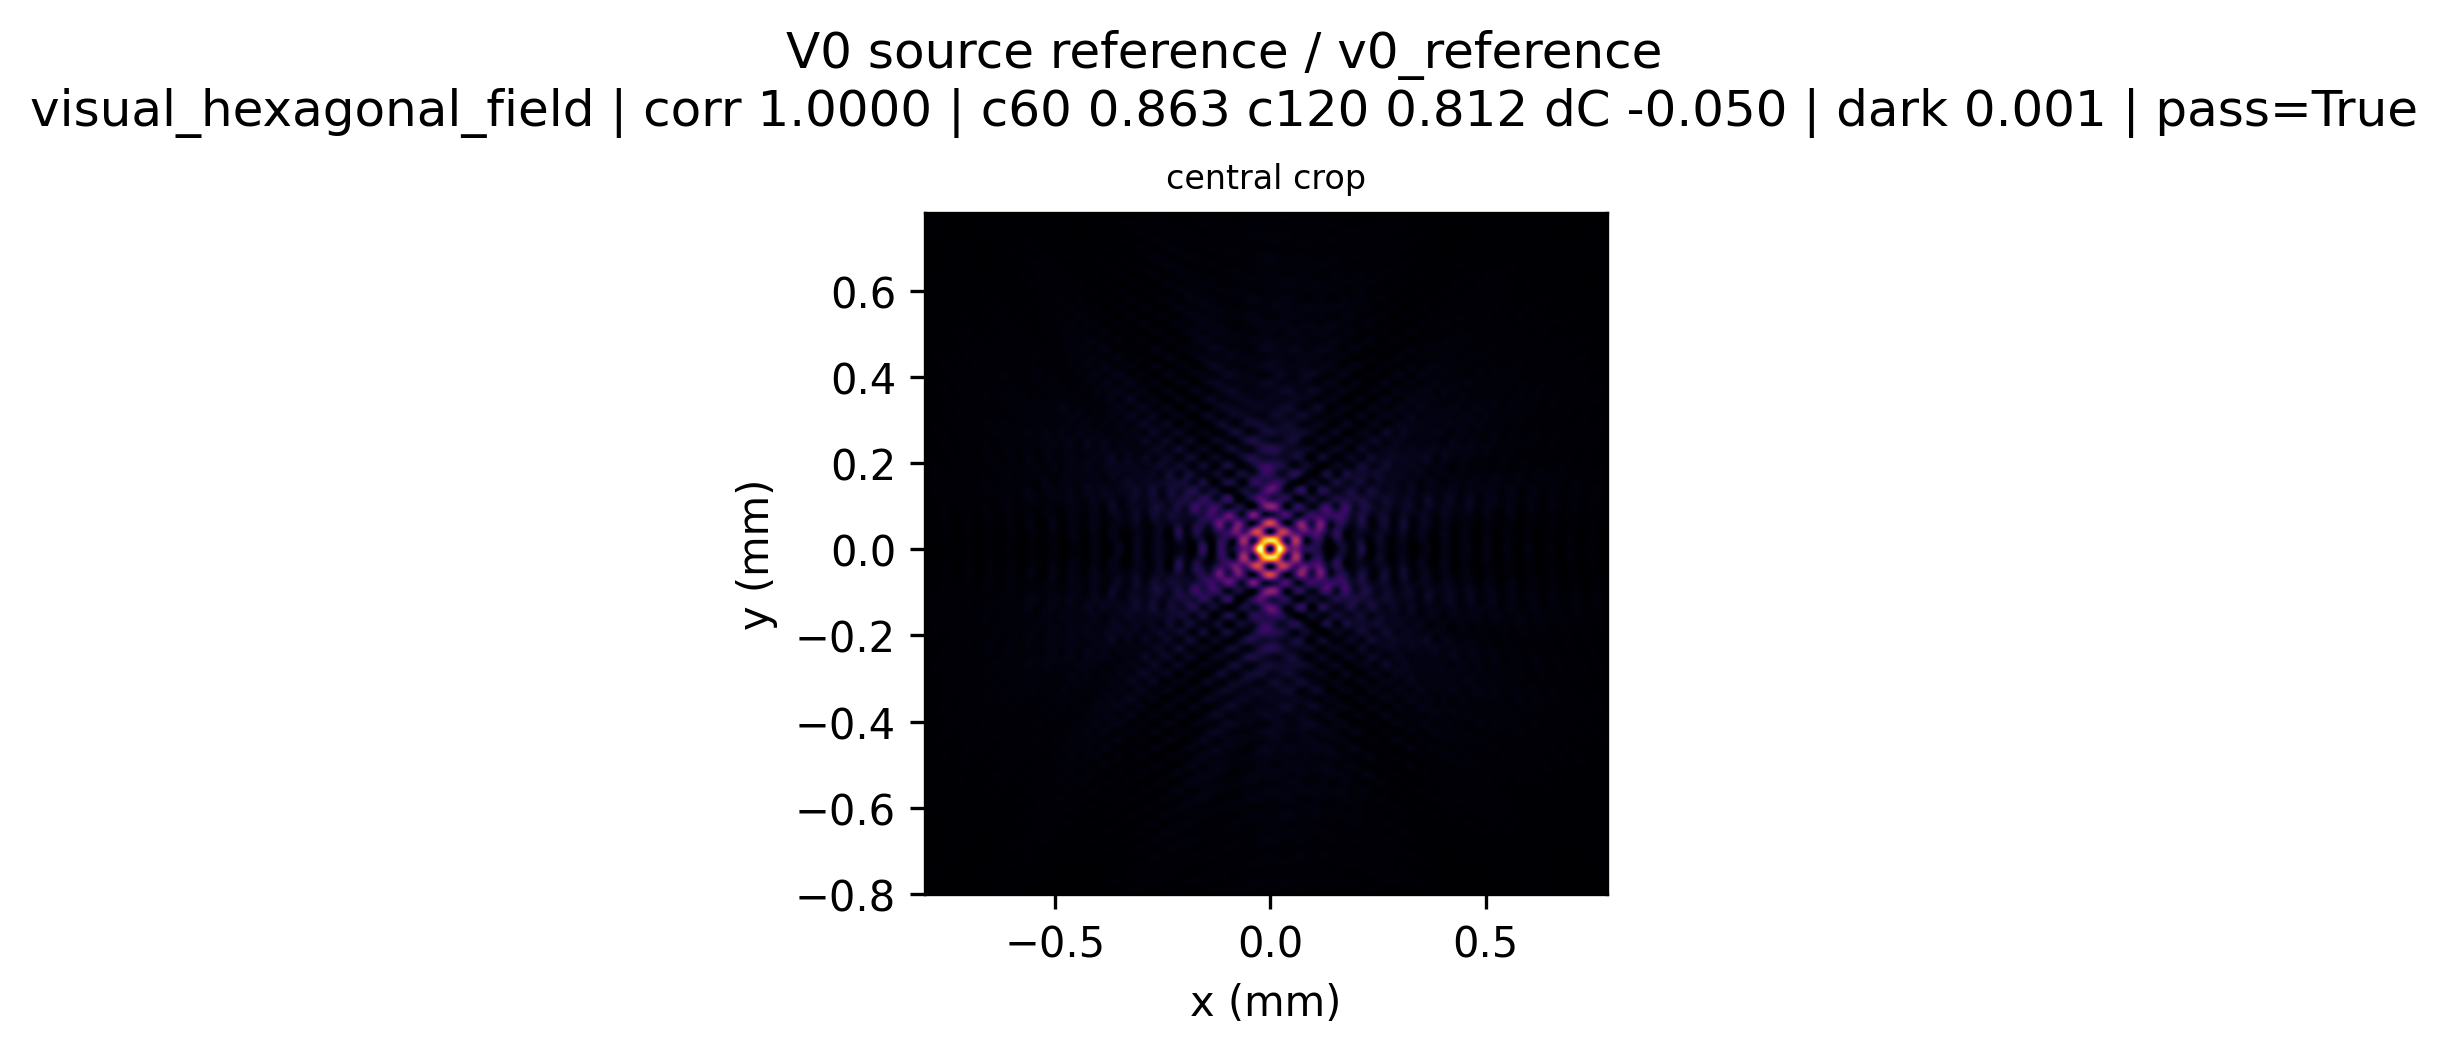
\includegraphics[width=\linewidth,height=0.82\textheight,keepaspectratio]{report/evidence_pack/source_validation/F03_v0_reference_crop_highres.png}
\caption{F03 (appendix): High-resolution V0 reference crop and propagated structure.}
\end{figure}

\begin{figure}[p]
\centering
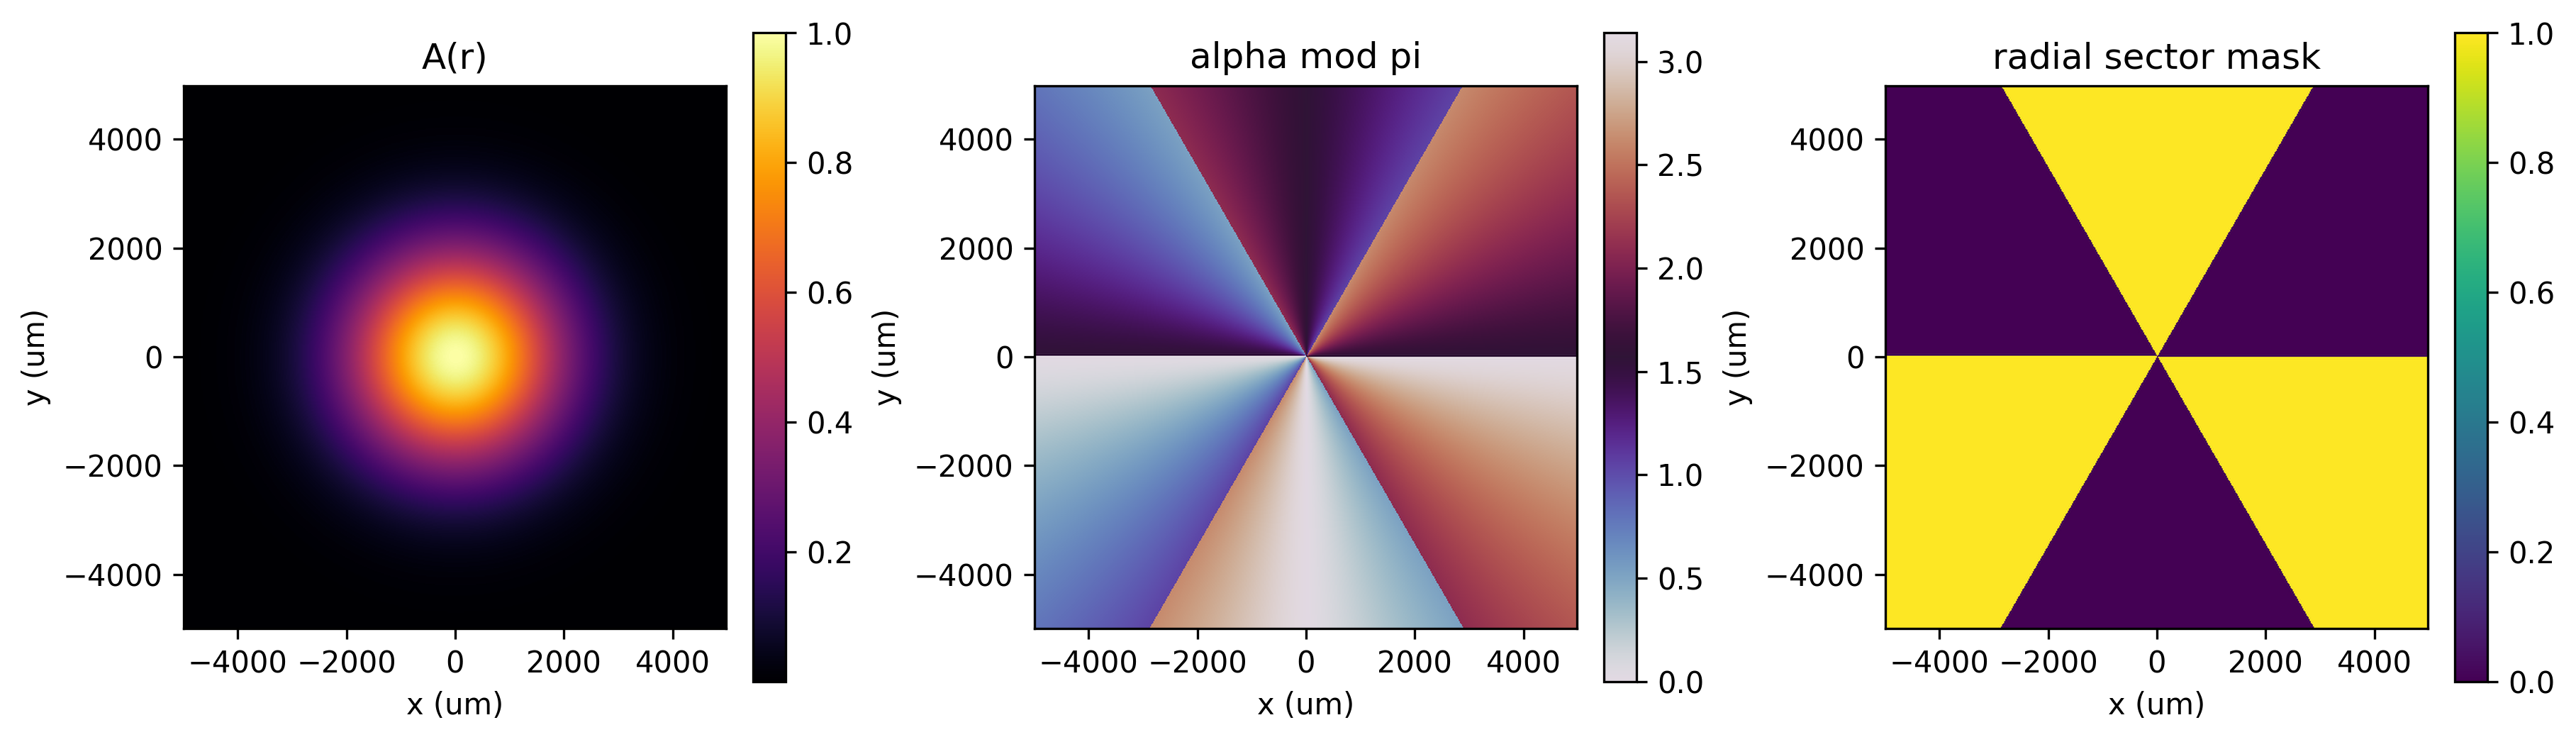
\includegraphics[width=\linewidth,height=0.82\textheight,keepaspectratio]{report/evidence_pack/equations/F04_m2p_target_alpha_sector_highres.png}
\caption{F04 (appendix): M2P target alpha and sector map.}
\end{figure}

\begin{figure}[p]
\centering
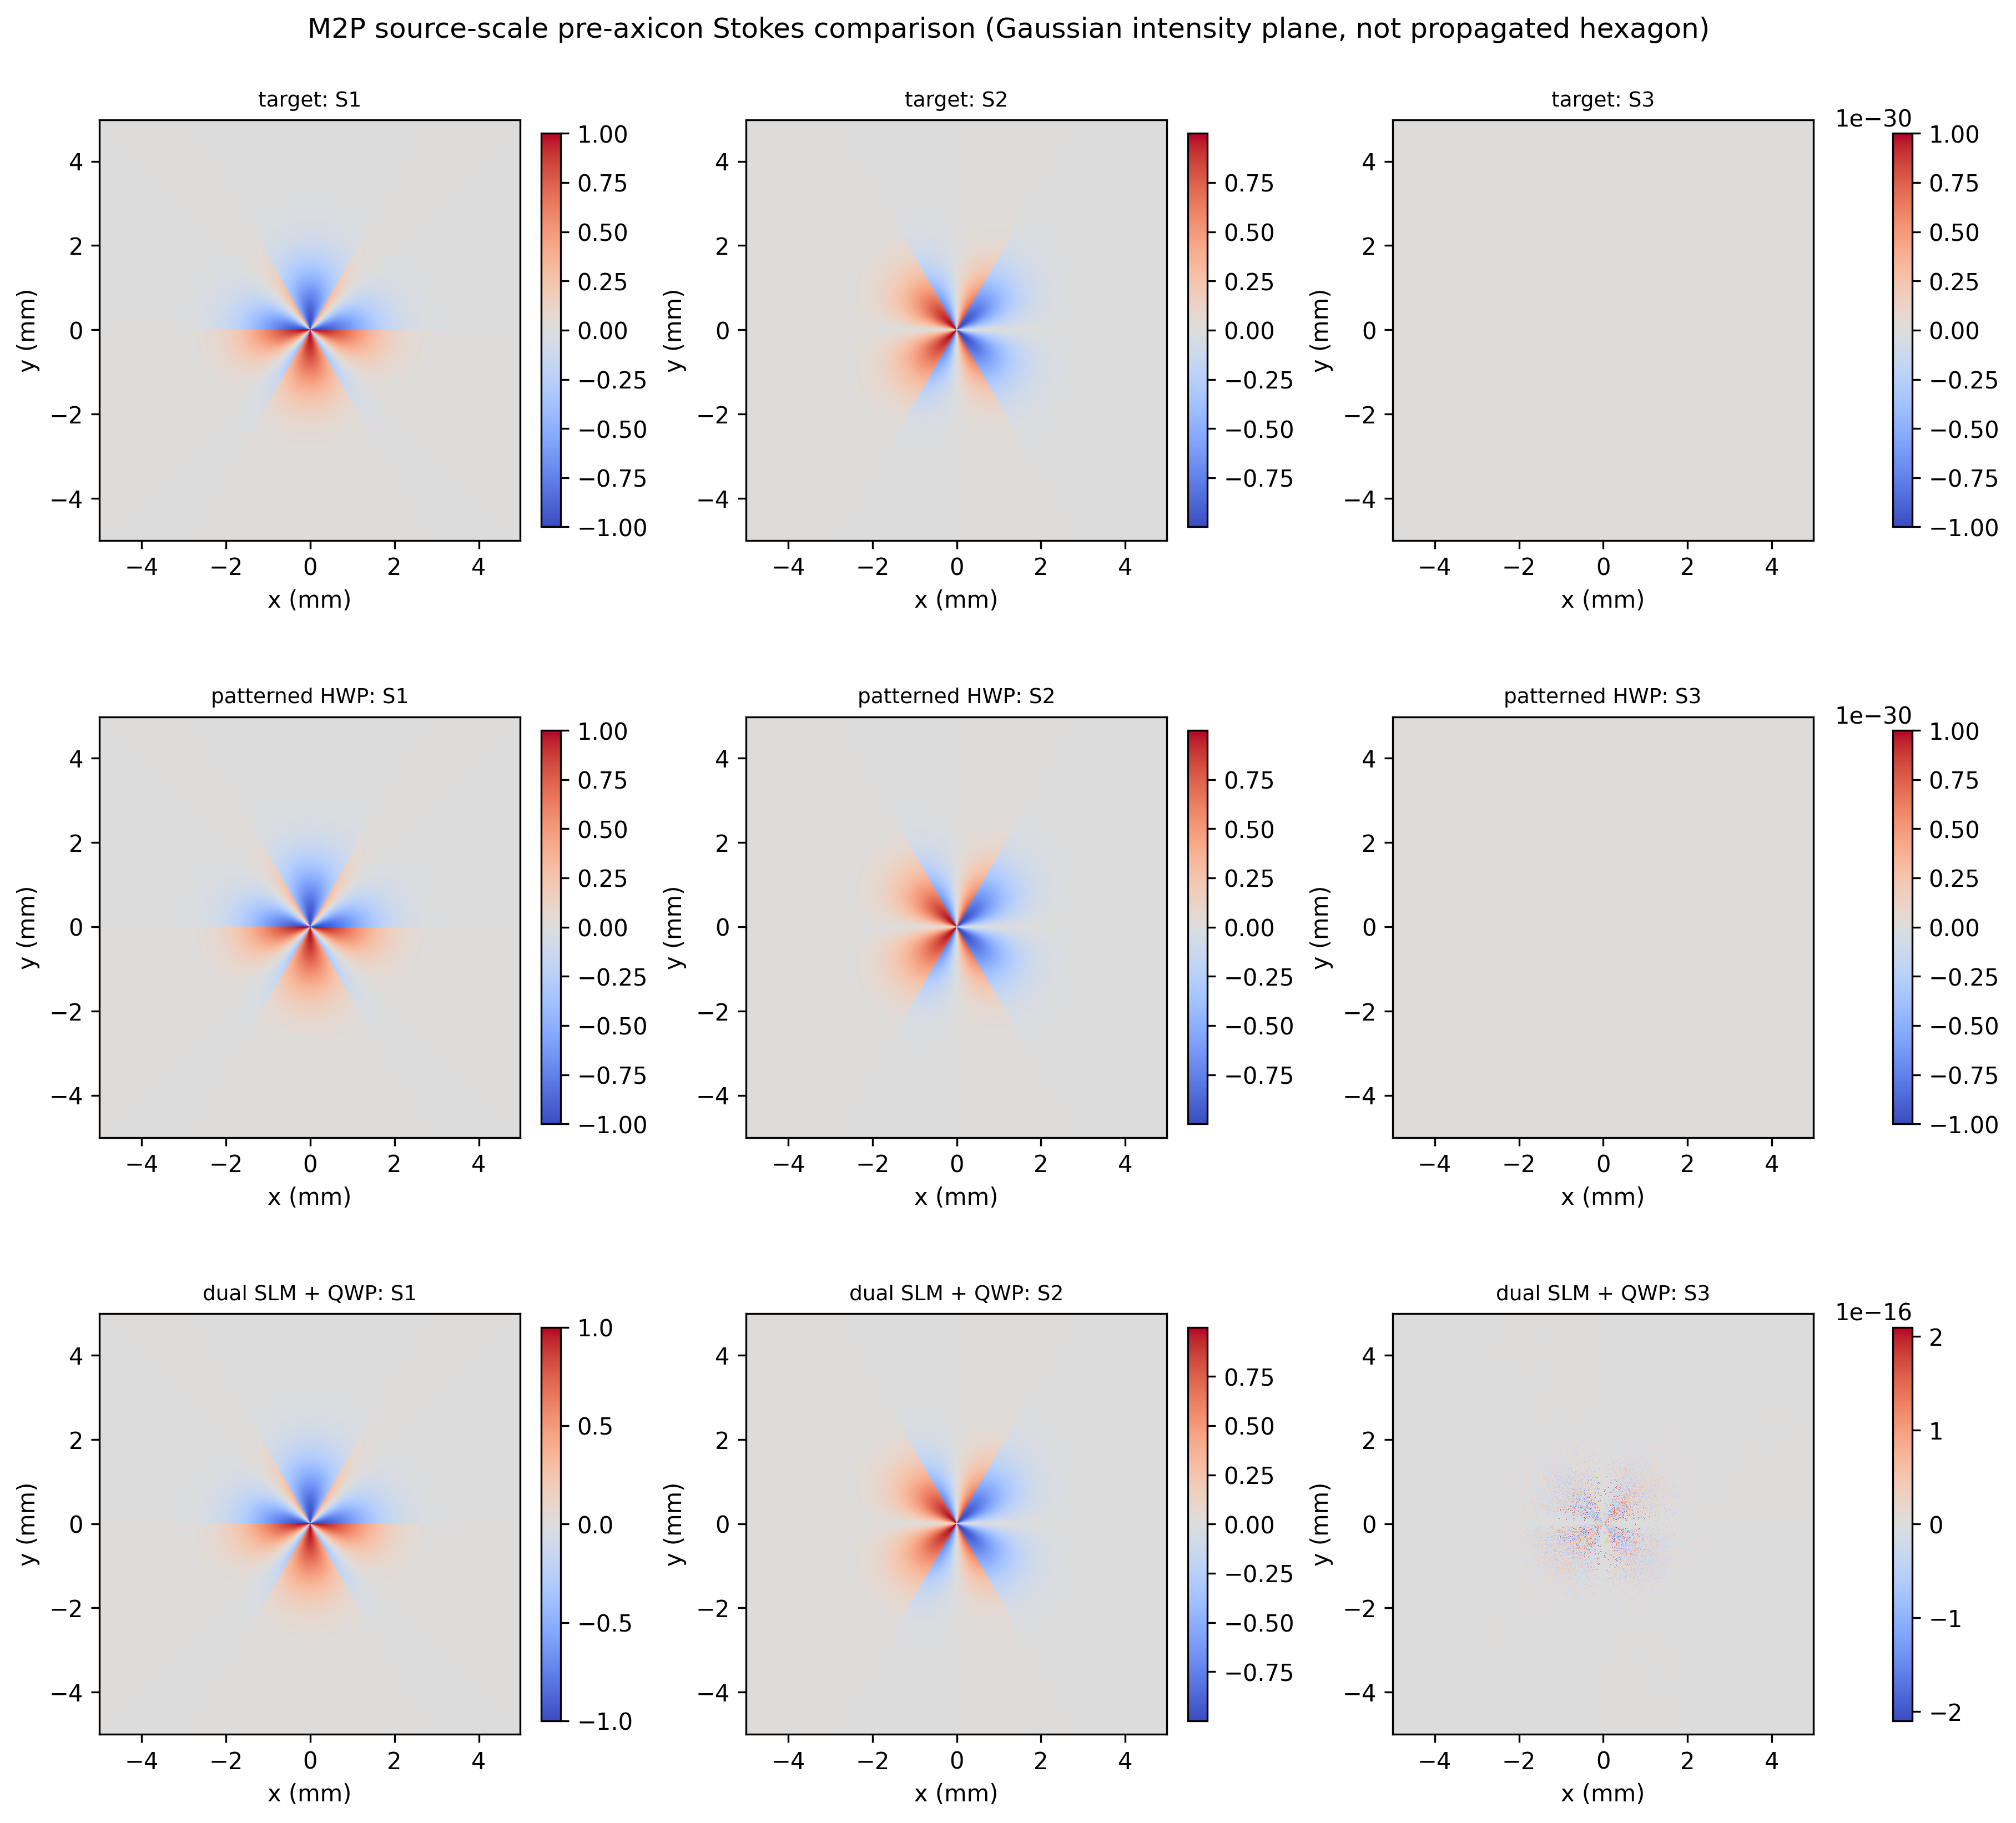
\includegraphics[width=\linewidth,height=0.82\textheight,keepaspectratio]{report/evidence_pack/equations/F05_m2p_stokes_comparison_highres.png}
\caption{F05 (appendix): M2P pre-axicon Stokes comparison.}
\end{figure}

\begin{figure}[p]
\centering
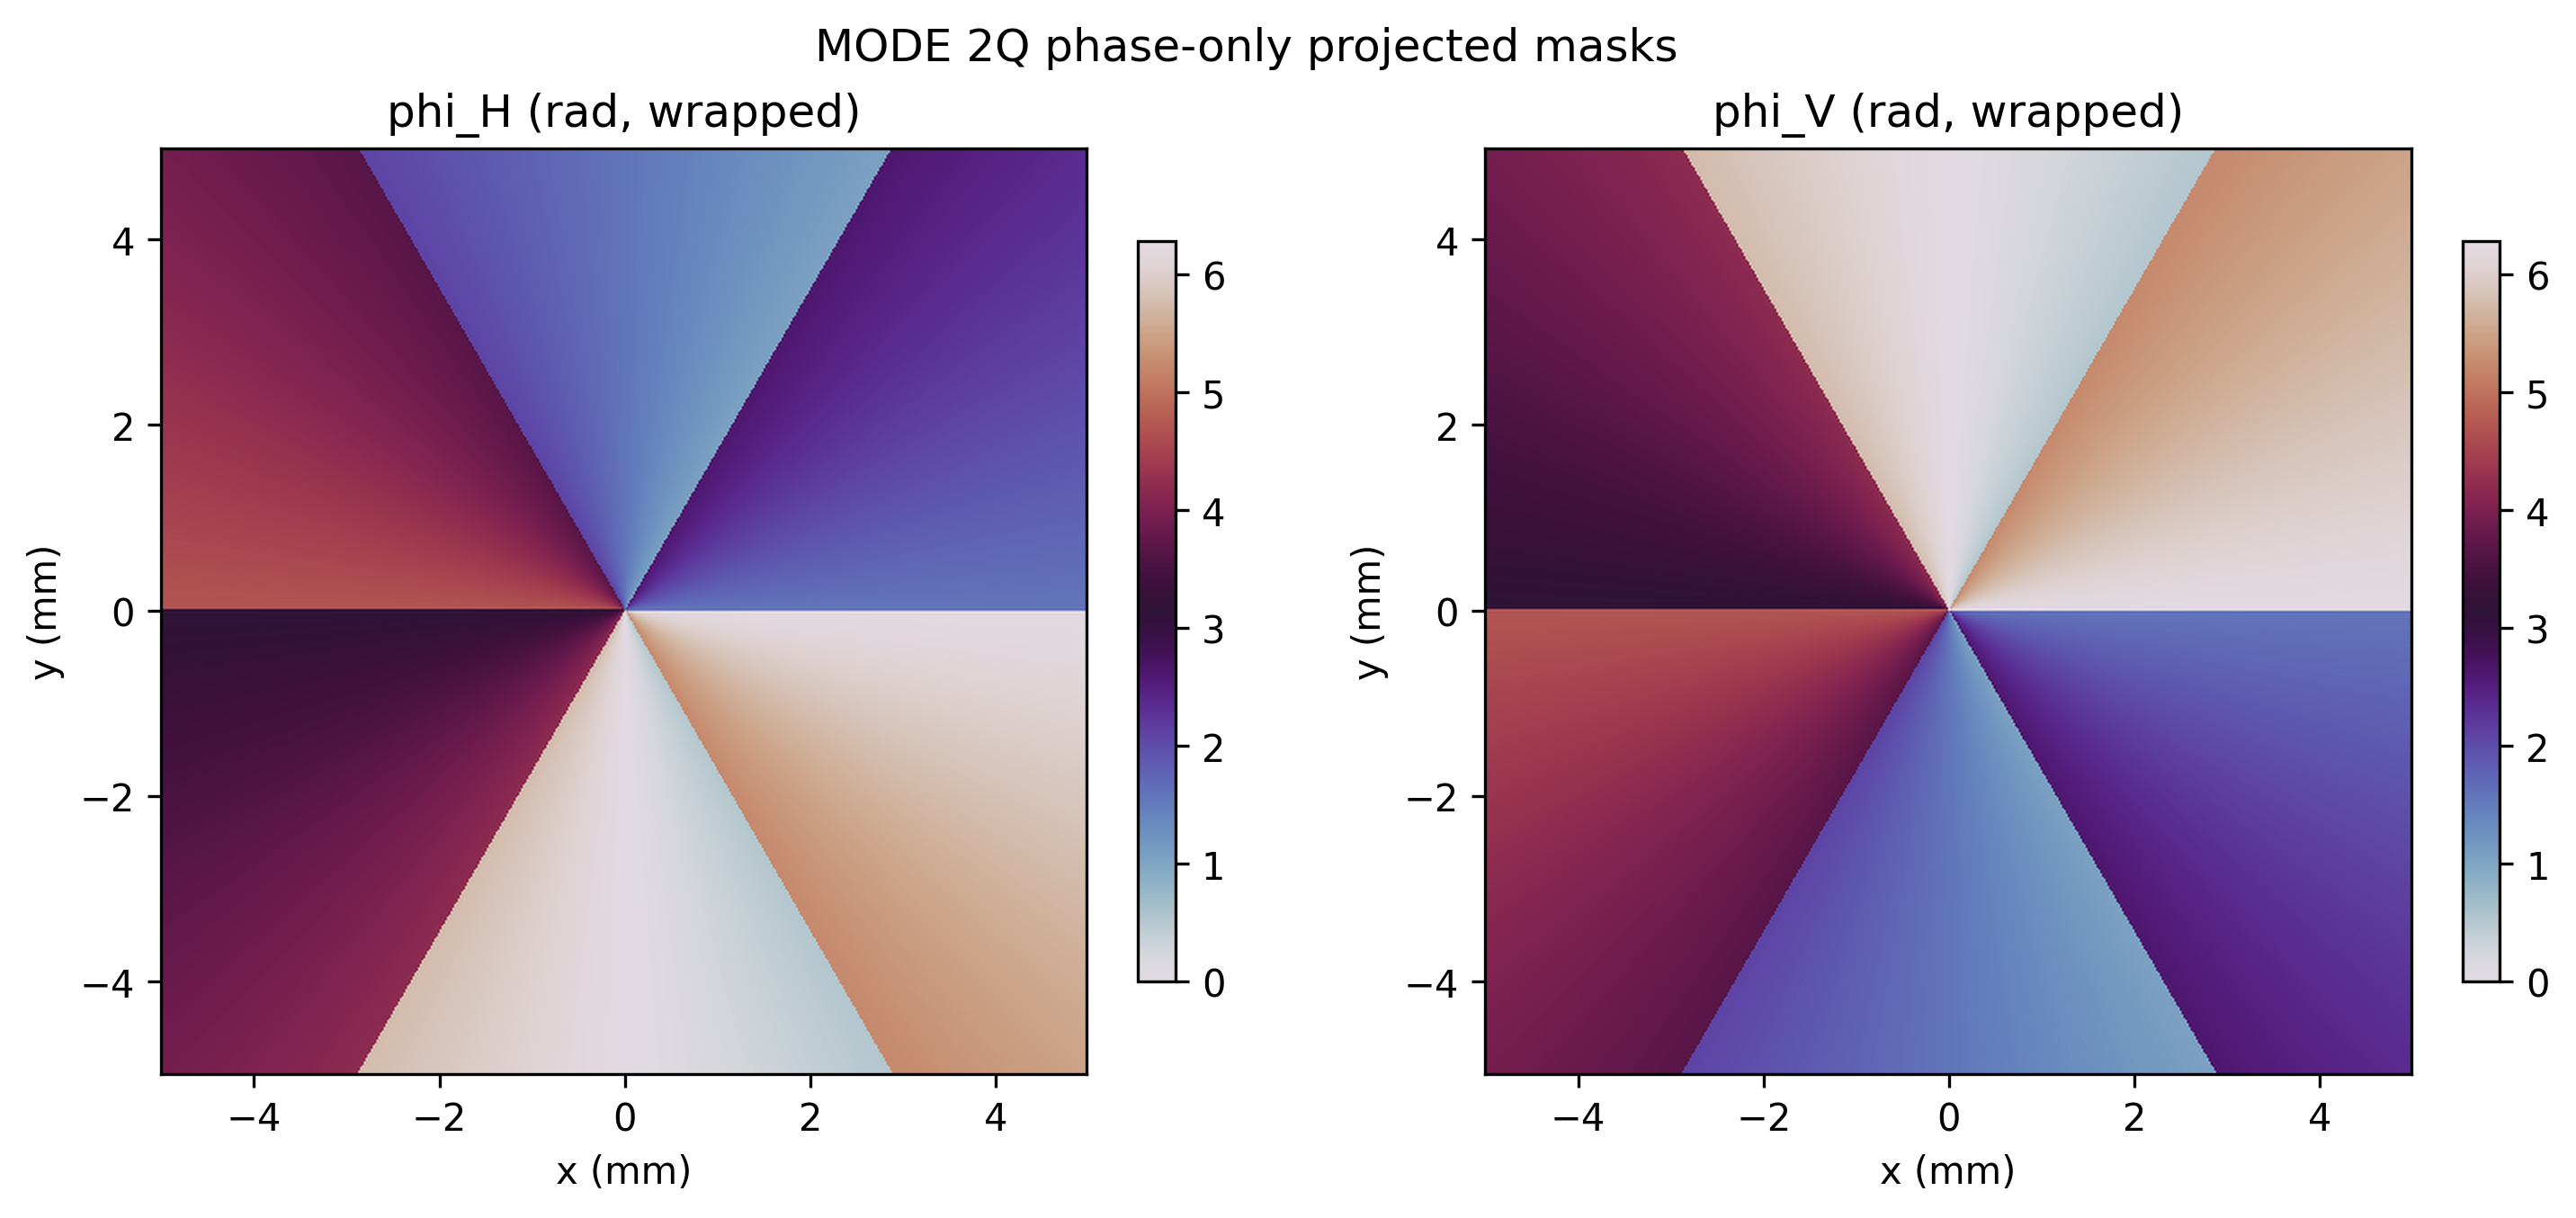
\includegraphics[width=\linewidth,height=0.82\textheight,keepaspectratio]{report/evidence_pack/inverse_design/F06_m2q_phase_only_masks_highres.png}
\caption{F06 (appendix): M2Q recovered phase-only masks and inverse design diagnostics.}
\end{figure}

\begin{figure}[p]
\centering
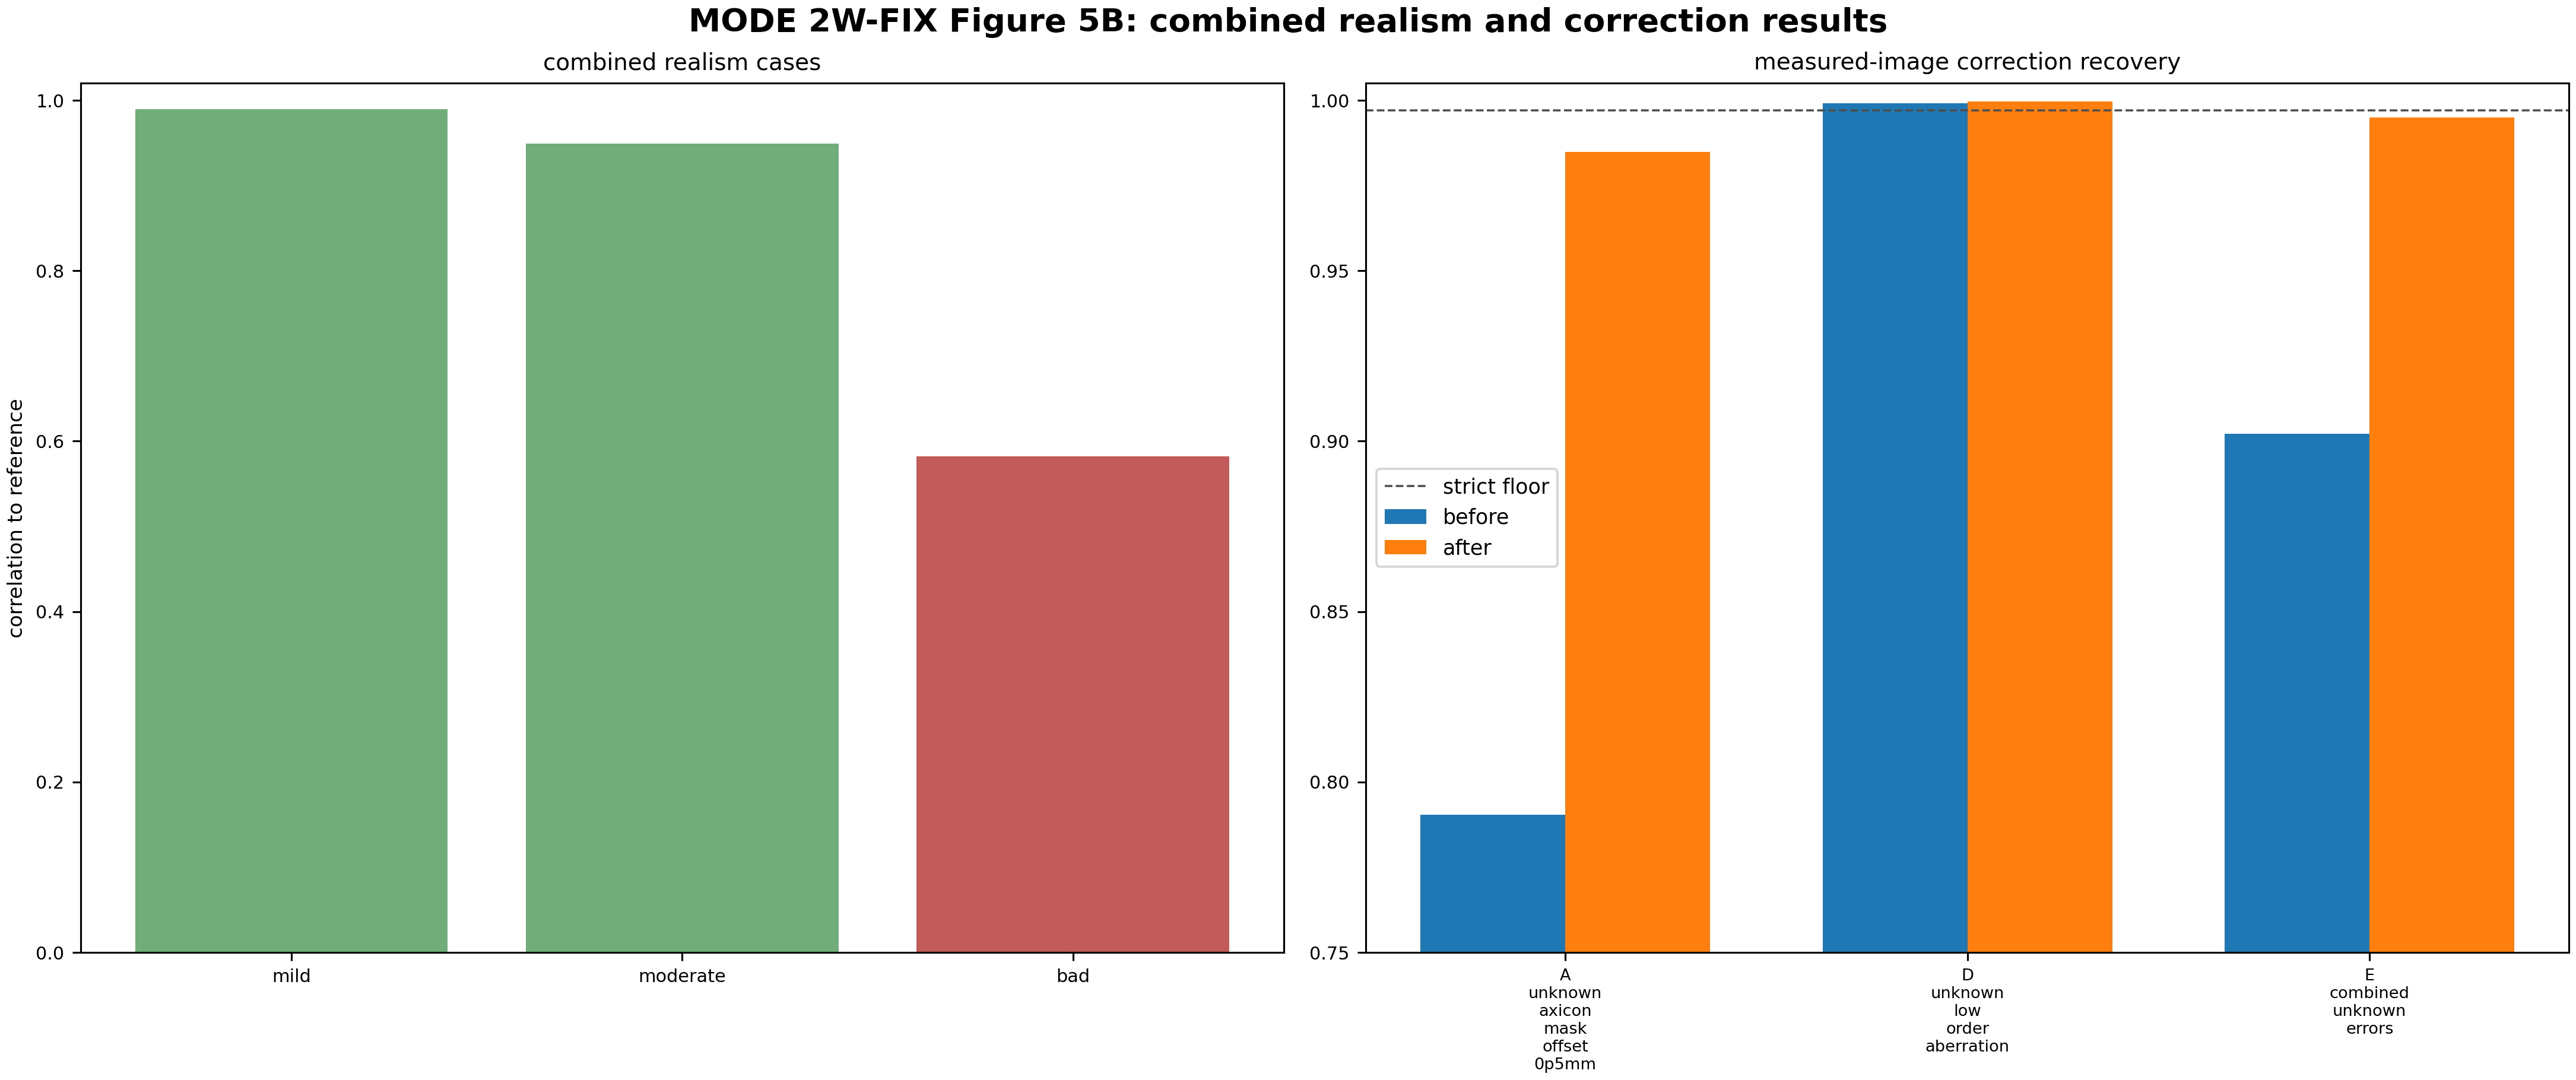
\includegraphics[width=\linewidth,height=0.82\textheight,keepaspectratio]{report/evidence_pack/correction/F16_fig5B_combined_correction_results.png}
\caption{F16 (appendix): Combined realism and correction results.}
\end{figure}

\begin{figure}[p]
\centering
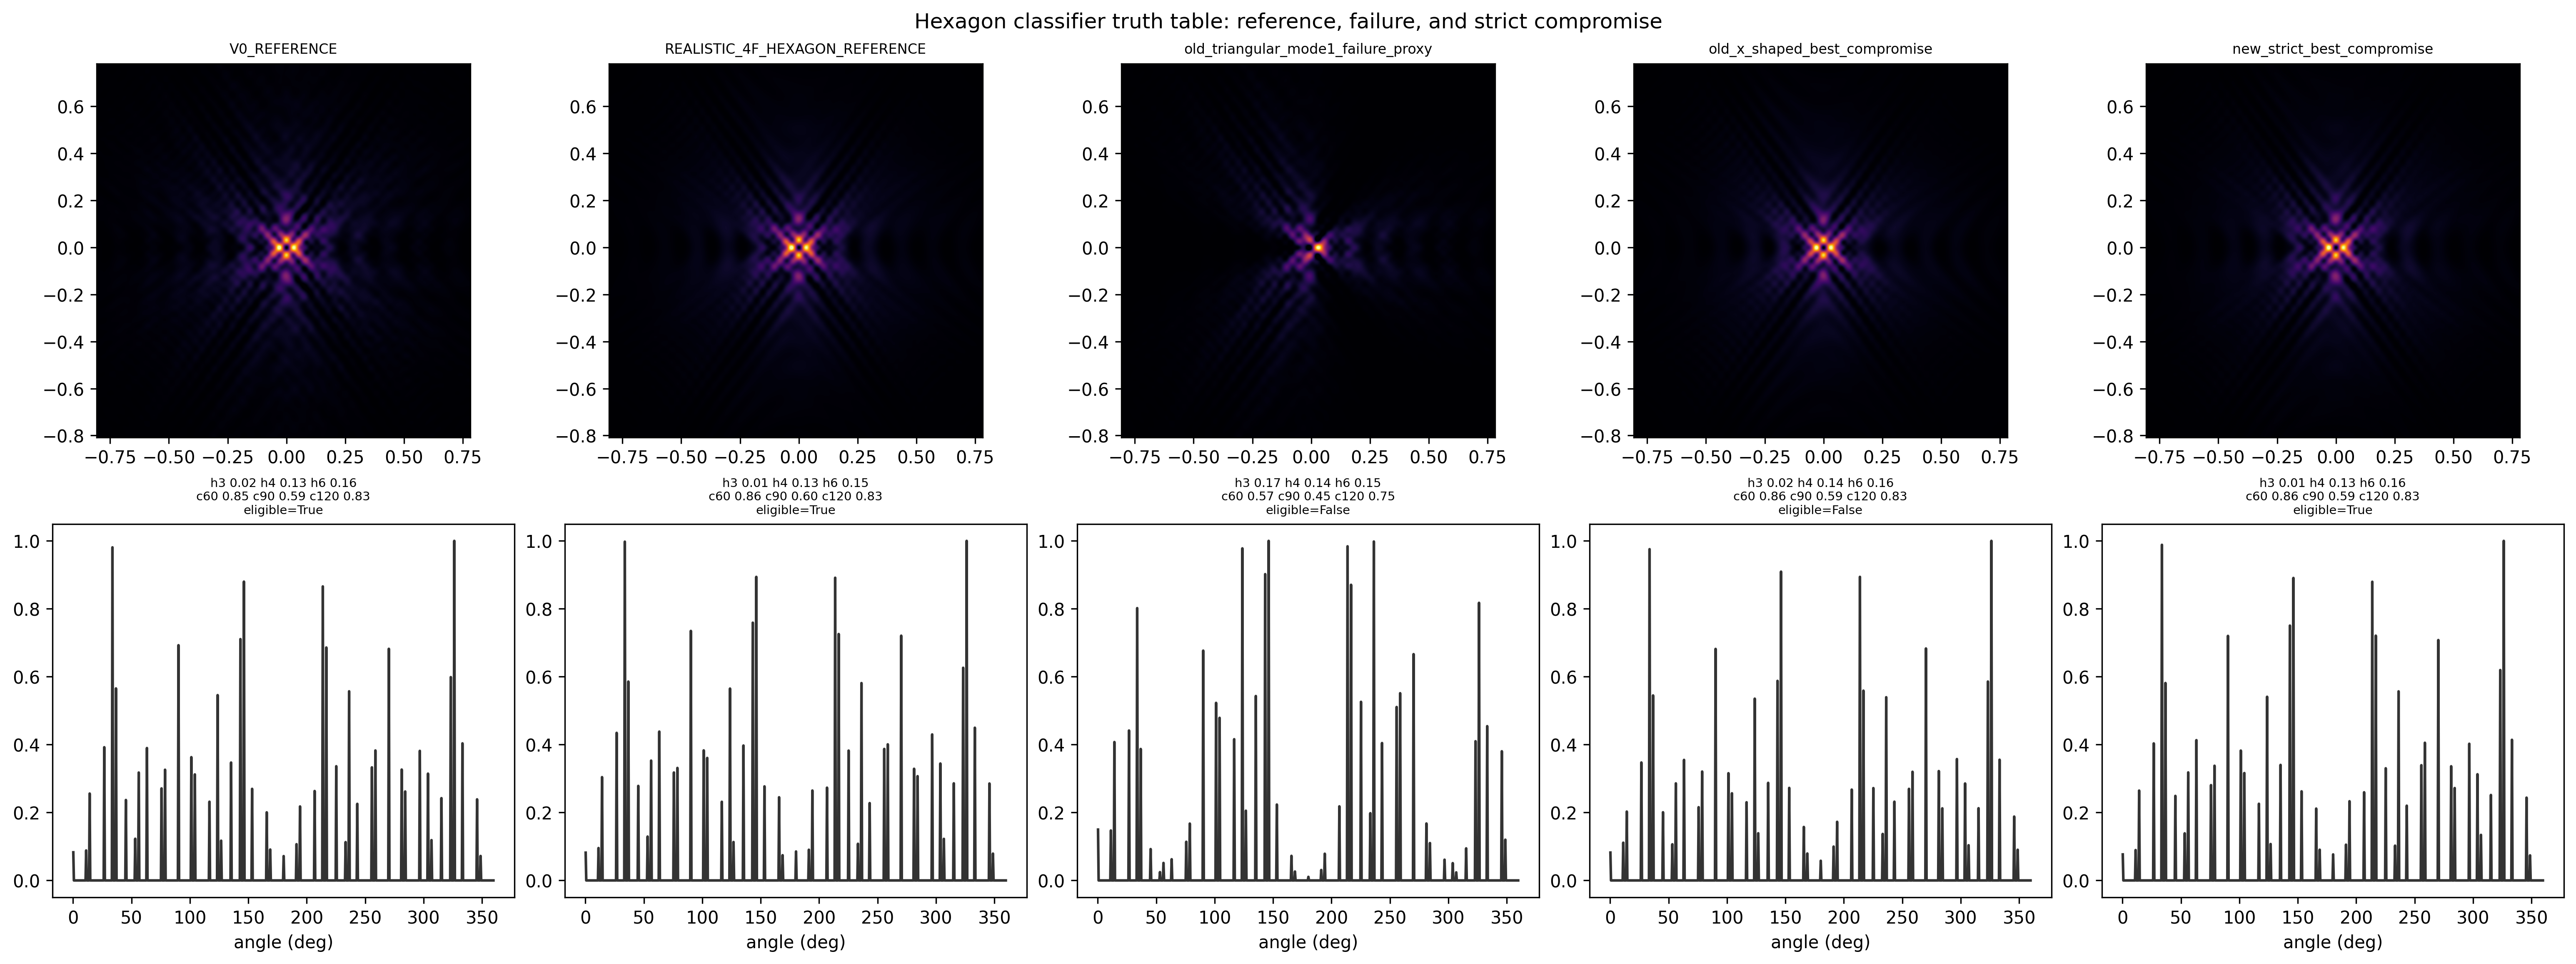
\includegraphics[width=\linewidth,height=0.82\textheight,keepaspectratio]{report/evidence_pack/provenance/F17_hexagon_classifier_truth_table_highres.png}
\caption{F17 (appendix): Strict classifier truth table and gate calibration.}
\end{figure}

\begin{figure}[p]
\centering
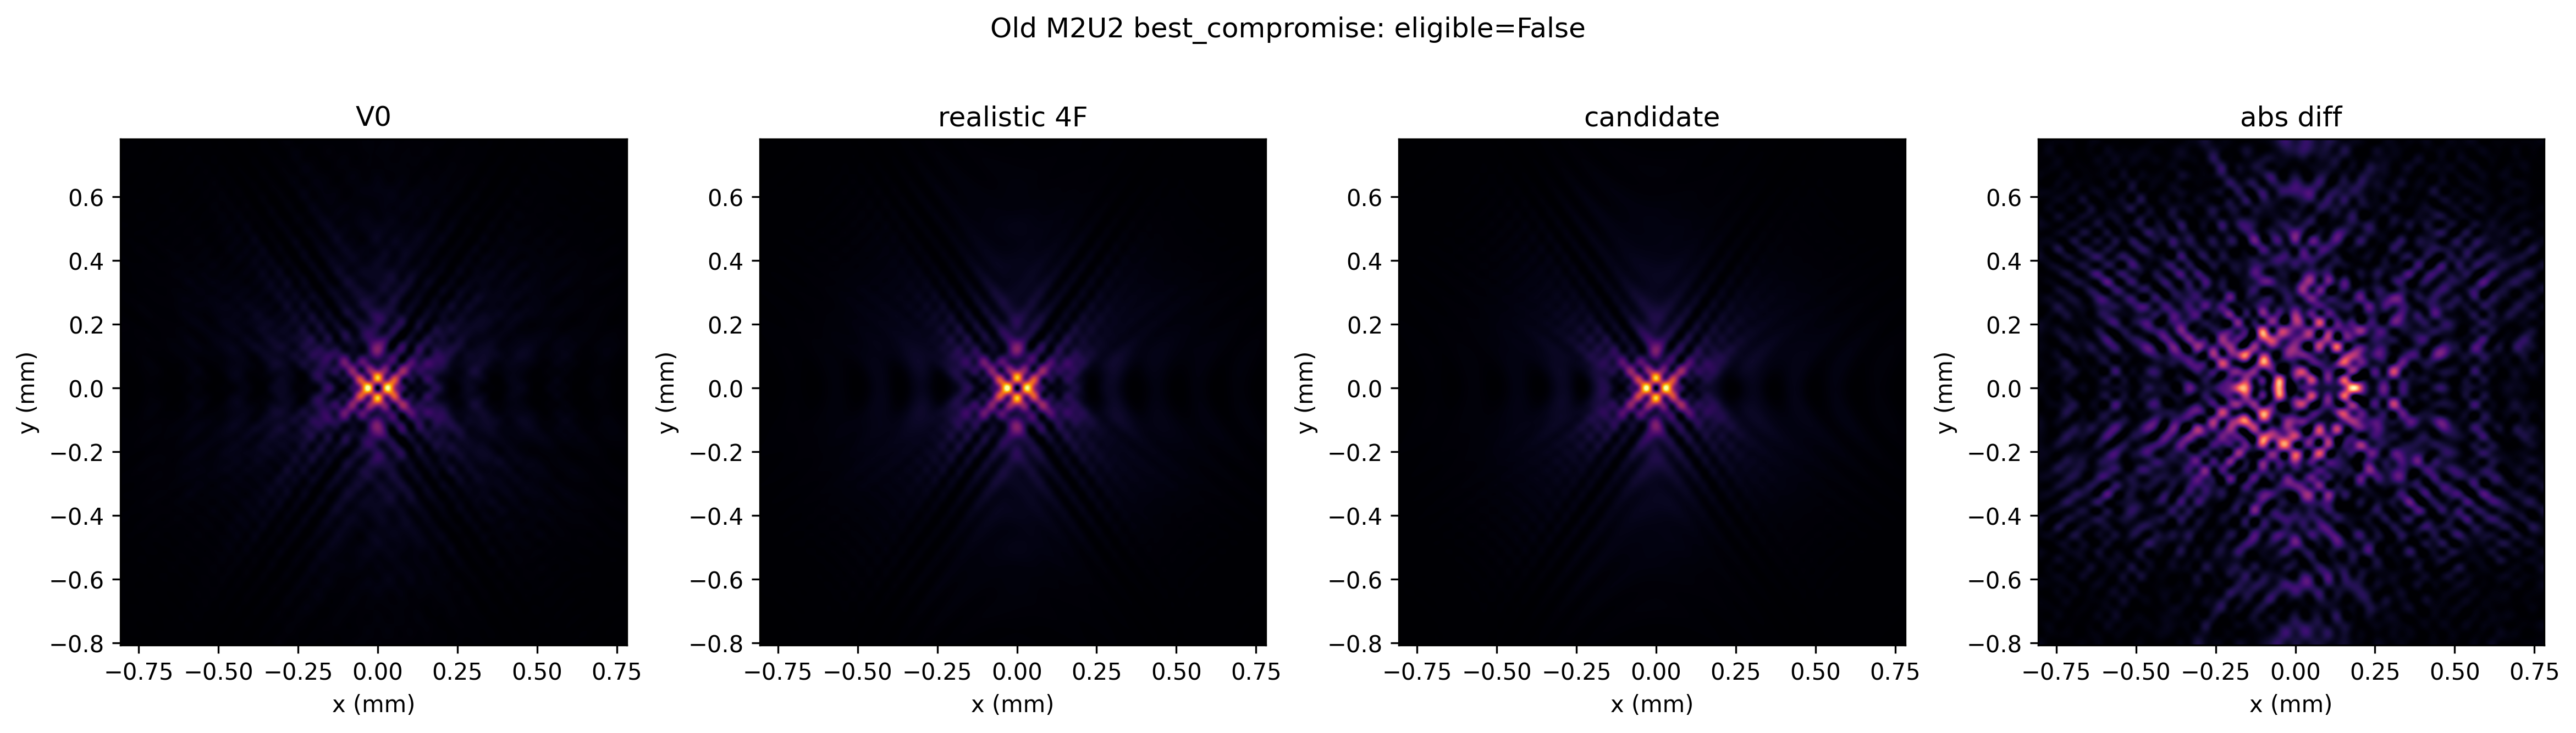
\includegraphics[width=\linewidth,height=0.82\textheight,keepaspectratio]{report/evidence_pack/superseded/S01_best_compromise_m2u2_opt_003_c5.75_i0.32_q-0.25_r+0.0_p0.10_audit.png}
\caption{S01 (appendix): Forbidden old best-compromise audit figure.}
\end{figure}

\end{document}